
\documentclass{article} % For LaTeX2e
\usepackage{iclr2021_conference,times}

\usepackage[utf8]{inputenc} % allow utf-8 input
\usepackage[T1]{fontenc}    % use 8-bit T1 fonts
\usepackage{hyperref}       % hyperlinks
\usepackage{url}            % simple URL typesetting
\usepackage{booktabs}       % professional-quality tables
\usepackage{amsfonts}       % blackboard math symbols
\usepackage{nicefrac}       % compact symbols for 1/2, etc.
\usepackage{xcolor}
\usepackage{ulem}

\usepackage{microtype}      % microtypography
\usepackage{amsmath}
\usepackage{graphicx}
\usepackage{arydshln}

\usepackage[lofdepth,lotdepth]{subfig}
\usepackage{pifont}

\newcommand{\Edouard}[1]{\textcolor{blue}{#1}}
\newcommand{\Louis}[1]{\textcolor{red}{#1}}
% Optional math commands from https://github.com/goodfeli/dlbook_notation.
%%%%% NEW MATH DEFINITIONS %%%%%

\usepackage{amsmath,amsfonts,bm}

% Mark sections of captions for referring to divisions of figures
\newcommand{\figleft}{{\em (Left)}}
\newcommand{\figcenter}{{\em (Center)}}
\newcommand{\figright}{{\em (Right)}}
\newcommand{\figtop}{{\em (Top)}}
\newcommand{\figbottom}{{\em (Bottom)}}
\newcommand{\captiona}{{\em (a)}}
\newcommand{\captionb}{{\em (b)}}
\newcommand{\captionc}{{\em (c)}}
\newcommand{\captiond}{{\em (d)}}

% Highlight a newly defined term
\newcommand{\newterm}[1]{{\bf #1}}


% Figure reference, lower-case.
\def\figref#1{figure~\ref{#1}}
% Figure reference, capital. For start of sentence
\def\Figref#1{Figure~\ref{#1}}
\def\twofigref#1#2{figures \ref{#1} and \ref{#2}}
\def\quadfigref#1#2#3#4{figures \ref{#1}, \ref{#2}, \ref{#3} and \ref{#4}}
% Section reference, lower-case.
\def\secref#1{section~\ref{#1}}
% Section reference, capital.
\def\Secref#1{Section~\ref{#1}}
% Reference to two sections.
\def\twosecrefs#1#2{sections \ref{#1} and \ref{#2}}
% Reference to three sections.
\def\secrefs#1#2#3{sections \ref{#1}, \ref{#2} and \ref{#3}}
% Reference to an equation, lower-case.
\def\eqref#1{equation~\ref{#1}}
% Reference to an equation, upper case
\def\Eqref#1{Equation~\ref{#1}}
% A raw reference to an equation---avoid using if possible
\def\plaineqref#1{\ref{#1}}
% Reference to a chapter, lower-case.
\def\chapref#1{chapter~\ref{#1}}
% Reference to an equation, upper case.
\def\Chapref#1{Chapter~\ref{#1}}
% Reference to a range of chapters
\def\rangechapref#1#2{chapters\ref{#1}--\ref{#2}}
% Reference to an algorithm, lower-case.
\def\algref#1{algorithm~\ref{#1}}
% Reference to an algorithm, upper case.
\def\Algref#1{Algorithm~\ref{#1}}
\def\twoalgref#1#2{algorithms \ref{#1} and \ref{#2}}
\def\Twoalgref#1#2{Algorithms \ref{#1} and \ref{#2}}
% Reference to a part, lower case
\def\partref#1{part~\ref{#1}}
% Reference to a part, upper case
\def\Partref#1{Part~\ref{#1}}
\def\twopartref#1#2{parts \ref{#1} and \ref{#2}}

\def\ceil#1{\lceil #1 \rceil}
\def\floor#1{\lfloor #1 \rfloor}
\def\1{\bm{1}}
\newcommand{\train}{\mathcal{D}}
\newcommand{\valid}{\mathcal{D_{\mathrm{valid}}}}
\newcommand{\test}{\mathcal{D_{\mathrm{test}}}}

\def\eps{{\epsilon}}


% Random variables
\def\reta{{\textnormal{$\eta$}}}
\def\ra{{\textnormal{a}}}
\def\rb{{\textnormal{b}}}
\def\rc{{\textnormal{c}}}
\def\rd{{\textnormal{d}}}
\def\re{{\textnormal{e}}}
\def\rf{{\textnormal{f}}}
\def\rg{{\textnormal{g}}}
\def\rh{{\textnormal{h}}}
\def\ri{{\textnormal{i}}}
\def\rj{{\textnormal{j}}}
\def\rk{{\textnormal{k}}}
\def\rl{{\textnormal{l}}}
% rm is already a command, just don't name any random variables m
\def\rn{{\textnormal{n}}}
\def\ro{{\textnormal{o}}}
\def\rp{{\textnormal{p}}}
\def\rq{{\textnormal{q}}}
\def\rr{{\textnormal{r}}}
\def\rs{{\textnormal{s}}}
\def\rt{{\textnormal{t}}}
\def\ru{{\textnormal{u}}}
\def\rv{{\textnormal{v}}}
\def\rw{{\textnormal{w}}}
\def\rx{{\textnormal{x}}}
\def\ry{{\textnormal{y}}}
\def\rz{{\textnormal{z}}}

% Random vectors
\def\rvepsilon{{\mathbf{\epsilon}}}
\def\rvtheta{{\mathbf{\theta}}}
\def\rva{{\mathbf{a}}}
\def\rvb{{\mathbf{b}}}
\def\rvc{{\mathbf{c}}}
\def\rvd{{\mathbf{d}}}
\def\rve{{\mathbf{e}}}
\def\rvf{{\mathbf{f}}}
\def\rvg{{\mathbf{g}}}
\def\rvh{{\mathbf{h}}}
\def\rvu{{\mathbf{i}}}
\def\rvj{{\mathbf{j}}}
\def\rvk{{\mathbf{k}}}
\def\rvl{{\mathbf{l}}}
\def\rvm{{\mathbf{m}}}
\def\rvn{{\mathbf{n}}}
\def\rvo{{\mathbf{o}}}
\def\rvp{{\mathbf{p}}}
\def\rvq{{\mathbf{q}}}
\def\rvr{{\mathbf{r}}}
\def\rvs{{\mathbf{s}}}
\def\rvt{{\mathbf{t}}}
\def\rvu{{\mathbf{u}}}
\def\rvv{{\mathbf{v}}}
\def\rvw{{\mathbf{w}}}
\def\rvx{{\mathbf{x}}}
\def\rvy{{\mathbf{y}}}
\def\rvz{{\mathbf{z}}}

% Elements of random vectors
\def\erva{{\textnormal{a}}}
\def\ervb{{\textnormal{b}}}
\def\ervc{{\textnormal{c}}}
\def\ervd{{\textnormal{d}}}
\def\erve{{\textnormal{e}}}
\def\ervf{{\textnormal{f}}}
\def\ervg{{\textnormal{g}}}
\def\ervh{{\textnormal{h}}}
\def\ervi{{\textnormal{i}}}
\def\ervj{{\textnormal{j}}}
\def\ervk{{\textnormal{k}}}
\def\ervl{{\textnormal{l}}}
\def\ervm{{\textnormal{m}}}
\def\ervn{{\textnormal{n}}}
\def\ervo{{\textnormal{o}}}
\def\ervp{{\textnormal{p}}}
\def\ervq{{\textnormal{q}}}
\def\ervr{{\textnormal{r}}}
\def\ervs{{\textnormal{s}}}
\def\ervt{{\textnormal{t}}}
\def\ervu{{\textnormal{u}}}
\def\ervv{{\textnormal{v}}}
\def\ervw{{\textnormal{w}}}
\def\ervx{{\textnormal{x}}}
\def\ervy{{\textnormal{y}}}
\def\ervz{{\textnormal{z}}}

% Random matrices
\def\rmA{{\mathbf{A}}}
\def\rmB{{\mathbf{B}}}
\def\rmC{{\mathbf{C}}}
\def\rmD{{\mathbf{D}}}
\def\rmE{{\mathbf{E}}}
\def\rmF{{\mathbf{F}}}
\def\rmG{{\mathbf{G}}}
\def\rmH{{\mathbf{H}}}
\def\rmI{{\mathbf{I}}}
\def\rmJ{{\mathbf{J}}}
\def\rmK{{\mathbf{K}}}
\def\rmL{{\mathbf{L}}}
\def\rmM{{\mathbf{M}}}
\def\rmN{{\mathbf{N}}}
\def\rmO{{\mathbf{O}}}
\def\rmP{{\mathbf{P}}}
\def\rmQ{{\mathbf{Q}}}
\def\rmR{{\mathbf{R}}}
\def\rmS{{\mathbf{S}}}
\def\rmT{{\mathbf{T}}}
\def\rmU{{\mathbf{U}}}
\def\rmV{{\mathbf{V}}}
\def\rmW{{\mathbf{W}}}
\def\rmX{{\mathbf{X}}}
\def\rmY{{\mathbf{Y}}}
\def\rmZ{{\mathbf{Z}}}

% Elements of random matrices
\def\ermA{{\textnormal{A}}}
\def\ermB{{\textnormal{B}}}
\def\ermC{{\textnormal{C}}}
\def\ermD{{\textnormal{D}}}
\def\ermE{{\textnormal{E}}}
\def\ermF{{\textnormal{F}}}
\def\ermG{{\textnormal{G}}}
\def\ermH{{\textnormal{H}}}
\def\ermI{{\textnormal{I}}}
\def\ermJ{{\textnormal{J}}}
\def\ermK{{\textnormal{K}}}
\def\ermL{{\textnormal{L}}}
\def\ermM{{\textnormal{M}}}
\def\ermN{{\textnormal{N}}}
\def\ermO{{\textnormal{O}}}
\def\ermP{{\textnormal{P}}}
\def\ermQ{{\textnormal{Q}}}
\def\ermR{{\textnormal{R}}}
\def\ermS{{\textnormal{S}}}
\def\ermT{{\textnormal{T}}}
\def\ermU{{\textnormal{U}}}
\def\ermV{{\textnormal{V}}}
\def\ermW{{\textnormal{W}}}
\def\ermX{{\textnormal{X}}}
\def\ermY{{\textnormal{Y}}}
\def\ermZ{{\textnormal{Z}}}

% Vectors
\def\vzero{{\bm{0}}}
\def\vone{{\bm{1}}}
\def\vmu{{\bm{\mu}}}
\def\vtheta{{\bm{\theta}}}
\def\va{{\bm{a}}}
\def\vb{{\bm{b}}}
\def\vc{{\bm{c}}}
\def\vd{{\bm{d}}}
\def\ve{{\bm{e}}}
\def\vf{{\bm{f}}}
\def\vg{{\bm{g}}}
\def\vh{{\bm{h}}}
\def\vi{{\bm{i}}}
\def\vj{{\bm{j}}}
\def\vk{{\bm{k}}}
\def\vl{{\bm{l}}}
\def\vm{{\bm{m}}}
\def\vn{{\bm{n}}}
\def\vo{{\bm{o}}}
\def\vp{{\bm{p}}}
\def\vq{{\bm{q}}}
\def\vr{{\bm{r}}}
\def\vs{{\bm{s}}}
\def\vt{{\bm{t}}}
\def\vu{{\bm{u}}}
\def\vv{{\bm{v}}}
\def\vw{{\bm{w}}}
\def\vx{{\bm{x}}}
\def\vy{{\bm{y}}}
\def\vz{{\bm{z}}}

% Elements of vectors
\def\evalpha{{\alpha}}
\def\evbeta{{\beta}}
\def\evepsilon{{\epsilon}}
\def\evlambda{{\lambda}}
\def\evomega{{\omega}}
\def\evmu{{\mu}}
\def\evpsi{{\psi}}
\def\evsigma{{\sigma}}
\def\evtheta{{\theta}}
\def\eva{{a}}
\def\evb{{b}}
\def\evc{{c}}
\def\evd{{d}}
\def\eve{{e}}
\def\evf{{f}}
\def\evg{{g}}
\def\evh{{h}}
\def\evi{{i}}
\def\evj{{j}}
\def\evk{{k}}
\def\evl{{l}}
\def\evm{{m}}
\def\evn{{n}}
\def\evo{{o}}
\def\evp{{p}}
\def\evq{{q}}
\def\evr{{r}}
\def\evs{{s}}
\def\evt{{t}}
\def\evu{{u}}
\def\evv{{v}}
\def\evw{{w}}
\def\evx{{x}}
\def\evy{{y}}
\def\evz{{z}}

% Matrix
\def\mA{{\bm{A}}}
\def\mB{{\bm{B}}}
\def\mC{{\bm{C}}}
\def\mD{{\bm{D}}}
\def\mE{{\bm{E}}}
\def\mF{{\bm{F}}}
\def\mG{{\bm{G}}}
\def\mH{{\bm{H}}}
\def\mI{{\bm{I}}}
\def\mJ{{\bm{J}}}
\def\mK{{\bm{K}}}
\def\mL{{\bm{L}}}
\def\mM{{\bm{M}}}
\def\mN{{\bm{N}}}
\def\mO{{\bm{O}}}
\def\mP{{\bm{P}}}
\def\mQ{{\bm{Q}}}
\def\mR{{\bm{R}}}
\def\mS{{\bm{S}}}
\def\mT{{\bm{T}}}
\def\mU{{\bm{U}}}
\def\mV{{\bm{V}}}
\def\mW{{\bm{W}}}
\def\mX{{\bm{X}}}
\def\mY{{\bm{Y}}}
\def\mZ{{\bm{Z}}}
\def\mBeta{{\bm{\beta}}}
\def\mPhi{{\bm{\Phi}}}
\def\mLambda{{\bm{\Lambda}}}
\def\mSigma{{\bm{\Sigma}}}

% Tensor
\DeclareMathAlphabet{\mathsfit}{\encodingdefault}{\sfdefault}{m}{sl}
\SetMathAlphabet{\mathsfit}{bold}{\encodingdefault}{\sfdefault}{bx}{n}
\newcommand{\tens}[1]{\bm{\mathsfit{#1}}}
\def\tA{{\tens{A}}}
\def\tB{{\tens{B}}}
\def\tC{{\tens{C}}}
\def\tD{{\tens{D}}}
\def\tE{{\tens{E}}}
\def\tF{{\tens{F}}}
\def\tG{{\tens{G}}}
\def\tH{{\tens{H}}}
\def\tI{{\tens{I}}}
\def\tJ{{\tens{J}}}
\def\tK{{\tens{K}}}
\def\tL{{\tens{L}}}
\def\tM{{\tens{M}}}
\def\tN{{\tens{N}}}
\def\tO{{\tens{O}}}
\def\tP{{\tens{P}}}
\def\tQ{{\tens{Q}}}
\def\tR{{\tens{R}}}
\def\tS{{\tens{S}}}
\def\tT{{\tens{T}}}
\def\tU{{\tens{U}}}
\def\tV{{\tens{V}}}
\def\tW{{\tens{W}}}
\def\tX{{\tens{X}}}
\def\tY{{\tens{Y}}}
\def\tZ{{\tens{Z}}}


% Graph
\def\gA{{\mathcal{A}}}
\def\gB{{\mathcal{B}}}
\def\gC{{\mathcal{C}}}
\def\gD{{\mathcal{D}}}
\def\gE{{\mathcal{E}}}
\def\gF{{\mathcal{F}}}
\def\gG{{\mathcal{G}}}
\def\gH{{\mathcal{H}}}
\def\gI{{\mathcal{I}}}
\def\gJ{{\mathcal{J}}}
\def\gK{{\mathcal{K}}}
\def\gL{{\mathcal{L}}}
\def\gM{{\mathcal{M}}}
\def\gN{{\mathcal{N}}}
\def\gO{{\mathcal{O}}}
\def\gP{{\mathcal{P}}}
\def\gQ{{\mathcal{Q}}}
\def\gR{{\mathcal{R}}}
\def\gS{{\mathcal{S}}}
\def\gT{{\mathcal{T}}}
\def\gU{{\mathcal{U}}}
\def\gV{{\mathcal{V}}}
\def\gW{{\mathcal{W}}}
\def\gX{{\mathcal{X}}}
\def\gY{{\mathcal{Y}}}
\def\gZ{{\mathcal{Z}}}

% Sets
\def\sA{{\mathbb{A}}}
\def\sB{{\mathbb{B}}}
\def\sC{{\mathbb{C}}}
\def\sD{{\mathbb{D}}}
% Don't use a set called E, because this would be the same as our symbol
% for expectation.
\def\sF{{\mathbb{F}}}
\def\sG{{\mathbb{G}}}
\def\sH{{\mathbb{H}}}
\def\sI{{\mathbb{I}}}
\def\sJ{{\mathbb{J}}}
\def\sK{{\mathbb{K}}}
\def\sL{{\mathbb{L}}}
\def\sM{{\mathbb{M}}}
\def\sN{{\mathbb{N}}}
\def\sO{{\mathbb{O}}}
\def\sP{{\mathbb{P}}}
\def\sQ{{\mathbb{Q}}}
\def\sR{{\mathbb{R}}}
\def\sS{{\mathbb{S}}}
\def\sT{{\mathbb{T}}}
\def\sU{{\mathbb{U}}}
\def\sV{{\mathbb{V}}}
\def\sW{{\mathbb{W}}}
\def\sX{{\mathbb{X}}}
\def\sY{{\mathbb{Y}}}
\def\sZ{{\mathbb{Z}}}

% Entries of a matrix
\def\emLambda{{\Lambda}}
\def\emA{{A}}
\def\emB{{B}}
\def\emC{{C}}
\def\emD{{D}}
\def\emE{{E}}
\def\emF{{F}}
\def\emG{{G}}
\def\emH{{H}}
\def\emI{{I}}
\def\emJ{{J}}
\def\emK{{K}}
\def\emL{{L}}
\def\emM{{M}}
\def\emN{{N}}
\def\emO{{O}}
\def\emP{{P}}
\def\emQ{{Q}}
\def\emR{{R}}
\def\emS{{S}}
\def\emT{{T}}
\def\emU{{U}}
\def\emV{{V}}
\def\emW{{W}}
\def\emX{{X}}
\def\emY{{Y}}
\def\emZ{{Z}}
\def\emSigma{{\Sigma}}

% entries of a tensor
% Same font as tensor, without \bm wrapper
\newcommand{\etens}[1]{\mathsfit{#1}}
\def\etLambda{{\etens{\Lambda}}}
\def\etA{{\etens{A}}}
\def\etB{{\etens{B}}}
\def\etC{{\etens{C}}}
\def\etD{{\etens{D}}}
\def\etE{{\etens{E}}}
\def\etF{{\etens{F}}}
\def\etG{{\etens{G}}}
\def\etH{{\etens{H}}}
\def\etI{{\etens{I}}}
\def\etJ{{\etens{J}}}
\def\etK{{\etens{K}}}
\def\etL{{\etens{L}}}
\def\etM{{\etens{M}}}
\def\etN{{\etens{N}}}
\def\etO{{\etens{O}}}
\def\etP{{\etens{P}}}
\def\etQ{{\etens{Q}}}
\def\etR{{\etens{R}}}
\def\etS{{\etens{S}}}
\def\etT{{\etens{T}}}
\def\etU{{\etens{U}}}
\def\etV{{\etens{V}}}
\def\etW{{\etens{W}}}
\def\etX{{\etens{X}}}
\def\etY{{\etens{Y}}}
\def\etZ{{\etens{Z}}}

% The true underlying data generating distribution
\newcommand{\pdata}{p_{\rm{data}}}
% The empirical distribution defined by the training set
\newcommand{\ptrain}{\hat{p}_{\rm{data}}}
\newcommand{\Ptrain}{\hat{P}_{\rm{data}}}
% The model distribution
\newcommand{\pmodel}{p_{\rm{model}}}
\newcommand{\Pmodel}{P_{\rm{model}}}
\newcommand{\ptildemodel}{\tilde{p}_{\rm{model}}}
% Stochastic autoencoder distributions
\newcommand{\pencode}{p_{\rm{encoder}}}
\newcommand{\pdecode}{p_{\rm{decoder}}}
\newcommand{\precons}{p_{\rm{reconstruct}}}

\newcommand{\laplace}{\mathrm{Laplace}} % Laplace distribution

\newcommand{\E}{\mathbb{E}}
\newcommand{\Ls}{\mathcal{L}}
\newcommand{\R}{\mathbb{R}}
\newcommand{\emp}{\tilde{p}}
\newcommand{\lr}{\alpha}
\newcommand{\reg}{\lambda}
\newcommand{\rect}{\mathrm{rectifier}}
\newcommand{\softmax}{\mathrm{softmax}}
\newcommand{\sigmoid}{\sigma}
\newcommand{\softplus}{\zeta}
\newcommand{\KL}{D_{\mathrm{KL}}}
\newcommand{\Var}{\mathrm{Var}}
\newcommand{\standarderror}{\mathrm{SE}}
\newcommand{\Cov}{\mathrm{Cov}}
% Wolfram Mathworld says $L^2$ is for function spaces and $\ell^2$ is for vectors
% But then they seem to use $L^2$ for vectors throughout the site, and so does
% wikipedia.
\newcommand{\normlzero}{L^0}
\newcommand{\normlone}{L^1}
\newcommand{\normltwo}{L^2}
\newcommand{\normlp}{L^p}
\newcommand{\normmax}{L^\infty}

\newcommand{\parents}{Pa} % See usage in notation.tex. Chosen to match Daphne's book.

\DeclareMathOperator*{\argmax}{arg\,max}
\DeclareMathOperator*{\argmin}{arg\,min}

\DeclareMathOperator{\sign}{sign}
\DeclareMathOperator{\Tr}{Tr}
\let\ab\allowbreak


\usepackage{hyperref}
\usepackage{url}


%\title{\Edouard{On the importance of data-driven features for unsupervised visual representation}}
%\title{\Louis{On the importance of the data in the design of unsupervised visual representations}}
%\title{\Edouard{On the Implicit Need of Data  for Convolutional Kernel Methods}}
%\title{\Eugene(?){ Identifying The Key Ingredient for High Performance Convolutional Kernel Methods}}
\title{\Edouard{ On the Implicit  Key Ingredient for High Performance Convolutional Kernel Methods}}
% Authors must not appear in the submitted version. They should be hidden
% as long as the \iclrfinalcopy macro remains commented out below.
% Non-anonymous submissions will be rejected without review.

\author{Antiquus S.~Hippocampus, Natalia Cerebro \& Amelie P. Amygdale \thanks{ Use footnote for providing further information
about author (webpage, alternative address)---\emph{not} for acknowledging
funding agencies.  Funding acknowledgements go at the end of the paper.} \\
Department of Computer Science\\
Cranberry-Lemon University\\
Pittsburgh, PA 15213, USA \\
\texttt{\{hippo,brain,jen\}@cs.cranberry-lemon.edu} \\
\And
Ji Q. Ren \& Yevgeny LeNet \\
Department of Computational Neuroscience \\
University of the Witwatersrand \\
Joburg, South Africa \\
\texttt{\{robot,net\}@wits.ac.za} \\
\AND
Coauthor \\
Affiliation \\
Address \\
\texttt{email}
}

% The \author macro works with any number of authors. There are two commands
% used to separate the names and addresses of multiple authors: \And and \AND.
%
% Using \And between authors leaves it to \LaTeX{} to determine where to break
% the lines. Using \AND forces a linebreak at that point. So, if \LaTeX{}
% puts 3 of 4 authors names on the first line, and the last on the second
% line, try using \AND instead of \And before the third author name.

\newcommand{\fix}{\marginpar{FIX}}
\newcommand{\new}{\marginpar{NEW}}

%\iclrfinalcopy % Uncomment for camera-ready version, but NOT for submission.
\begin{document}
\maketitle

\begin{abstract}
A recent line of work showed that  various forms of convolutional  kernel methods can be competitive with standard supervised deep convolutional networks on datasets like CIFAR-10, obtaining accuracies in the range of $87-90\%$ while being more amenable to theoretical analysis. \Edouard{Here, we highlight that in order to get good performances,} these methods \Edouard{have to } rely \Edouard{explicitly} on a step that extracts features \Edouard{based on data from the training set, like dictionary of patches}. Here we extensively study its effect, demonstrating it is the key ingredient for high performance of these methods. Specifically, we show that \Edouard{one of the simplest data-driven kernel,} a method based on a \Edouard{single layer of }dictionary of patches, combined solely with a linear classifier is already obtaining classification accuracies in this range on CIFAR-10. We scale this method to the challenging ImageNet dataset, showing such a simple approach can exceed all existing non-learned representation methods. This is a new baseline for object recognition without representation learning methods, that  initiates the investigation of  convolutional kernel models  on ImageNet. We conduct experiments to analyze the dictionary that we used, our ablations showing that whitened patches are \Edouard{a key ingredient} for the success of this  type of method. 

%\color{red}{Eugene:  Several recent work towards understanding deep learning and building more principled deep learning models have focused on constructing models for the image classification setting. These models typically share aspects of deep convolutional networks used in practice while being more amenable to theoretical analysis. Although the performance gap of these models has decreased one can observe they all share as a typical preprocessing step the extraction of features based on random patches from natural images. Although characterized as a non-critical step, in this work we investigate the role of this patch based feature extraction finding that it is the primary driver of high performance. Indeed we observe that one can recover 86.5 \% on the CIFAR-10 dataset using just a method which matches patches in an image to nearest neighbors. Subsequently we ask what is hte limit of such an approach on a large scale dataset such as imagenet, finding that it can obtain performance compatible to methods relying on sophisticated image processign algorithm}
 
\end{abstract}

\section{Introduction}
% this paragraph must motivate why image classification analysis is difficult and the fact  that performance is one of the criterium used by researchers, that should be on imagenet - I think now it's good and clear
Understanding the success of deep convolutional neural networks on images has received a plethora of interest from the machine learning community. 
This is challenging because images are high-dimensional signals and deep neural networks are highly-non linear models  with a substantial amount of parameters: yet, the curse of dimensionality is seemingly avoided by these models. One approach taken by several authors \citep{mairal2016end,li2019enhanced,shankar2020neural,lu2014scale}  has been to construct simpler models that can achieve similar performance with a model that has more tractable analytical properties \citep{jacot2018neural,rahimi2008random}, but at the same time shares various elements with standard deep learning models. In general, these works are able to achieve reasonable performance on the CIFAR-10 dataset but lack of large scale experiments on datasets such as ImageNet.

%These analysis are thus difficult, and  their final conclusions are often relayed to obtaining  good  performances on standard benchmarks. Furthermore, there  exists generally a substential gap  of performances between the numerical experiments of works based on theorertical considerations and heavily engineered pipelines \citep{krizhevsky2012imagenet}. Several recent works have aimed to close this gap, attempting to provide models that have approachable theoretical properties but still providing a high performance
%~\citep{li2019enhanced,shankar2020neural}. %Yet, in general, they lack of large scale experiments on datasets such as ImageNet.

% This paragraph must discuss a/ the fact that a lot of theoretical(eg arora)/empirical(eg bagnet) works are implicitely or explicitely patch based b/ They don't do the necessary ablations to see that and the low dimensional structure of patches is quite more reasonable idea
% \mynotes{need a better flow above to not make the next sentecne repettivie}


%\paragraph{Deep convolutional kernel methods}Our work is primarily motivated by  the recent line of research which focuses on (potentially deep) convolutional kernels methods.
%These works rely on a common data-driven pre-processing step to construct a similarity measure at the image patch level. In this work we emphasize that there is a significant gap of performances if this pre-processing step is not used. We thus investigate to what extent this common step is responsible for the success of those methods, by considering a single layer model.
%We thus investigate the common step amongst these works, which all rely on similarity measure at the image patch level, finding this might be implicitely the reason of  their success.
%\Edouard{Indeed, \sout{w}ithout} clear ablation experiments, it remains difficult to know which design choices here are important, between the kernel design and the patch similarity measure. In our work, we decompose and analyze each step of our feature design, on gold-standard datasets and find that a method based solely on patches \Edouard{E: on garde?}$K$-Nearest Neighbors encoding in a dictionary of randomly selected patches is actually a strong baseline for image classification. 
%Those findings are aligned with empirical studies that relate deep learning models decisions with visual interpretations at small and large patch level
%\citep{zeiler2014visualizing,brendel2019approximating}.
%, which suggests that a subset of patches encodes much of the information of the class of an image.




%\subsection*{\Edouard{Work hypothesis}}
%\label{related_work}
 %We then propose a simple method in \ref{knn} to obtain an effective data-driven convolutional kernels for image classification while still being scalable.
%\subsection{Data-driven  kernels}\label{sec:data-driven_kernels}
%\Edouard{Linear or kernel methods rely heavily on the quality of the features which are fed to such algorithms. One observation of our work is that there is a substantial gap of performances between hand-crafted features and data-driven features. We believe our method remains simple because it does not involve any representation-learning step and thus no weight of our feature is adapted to a specific bias of the dataset. Furthermore, compared to deep method, ours is shallow.}
\paragraph{Data driven kernels} We first discuss the notion of  data-driven representations, which we believe is responsible for several competitive performances on simple image classification tasks.  We denote $\mathcal{X}$ the training set and we focus on \textit{standardized} representations which are fed to any predefined kernel $k$, such as a linear or Gaussian SVM, or even a random Neural Network. In other words, we consider similarity measures $\langle .,.\rangle_{k,\Phi,\mathcal{X}}$ that can be written:
\[\langle x,y\rangle_{k,\Phi,\mathcal{X}} =\langle L\Phi x,L\Phi y\rangle_k\, ,\]
where, we write here explicitely the dependency, $L=L(\Phi,\mathcal{X})$ is a diagonal affine operator and $\Phi x= \Phi(\mathcal{X},x)$. Standardization is mainly necessary for the optimization step, as it just corresponds to a rescaling of the data. It is said to be \textit{data-independent} if $\Phi$ does not depend on $\mathcal{X}$, and \textit{data-driven} otherwise. This, for instance, is the case if a dictionary  computed from the data \cite{li2019enhanced,mairal2016end} or a ZCA \cite{shankar2020neural} is incorporated in this representation. One of the goal of this paper is to clearly state that  kernel methods for vision do require to be data-driven and this is explicitely responsible for their success. We thus investigate to what extent this common step is responsible for the success of those methods, by considering a single layer model.

\paragraph{Work hypothesis}Our  methodology is based on ablation experiments: we would like to measure the effect of incorporating data, while reducing other side effects related to the design of $\Phi$, such as the depth of $\Phi$ or the implicit bias of a potential optimization procedure. Consequently, we focus on 1-hidden layer neural networks of any widths, which have favorable properties, like the ability to be a universal approximator under non-restrictive conditions. The output linear layer shall be optimized for a classification task, and we consider first layers which are predefined and kept fixed, similarly to \cite{coates2011analysis}. We will see below that simply initializing the weights of the first layer with patches leads to a significant gap of performances, compared to a random  initialization, a wavelet initialization or even a learning procedure. This patch initialization is used by several works \cite{li2019enhanced,mairal2016end} and is implicitly responsible for their good performances. Informally, this method can be thought as one of the simplest possible in the context of deep convolutional kernel methods, and we show that the depth or the non-linearities of such kernels play a minor role compared to the use of patches. In our work, we decompose and analyze each step of our feature design, on gold-standard datasets and find that a method based solely on patches and simple non-linearities is actually a strong baseline for image classification. 

%: we had to chose carefully a class of model as simple as possible. Thus, we focused on single layer architecture, which are in general better understood \citep{}, and we show that only the use of predefined randomly chosen patches from the training data is necessary to obtain non-trivial performances. We note that the method that we describe next involves no learning and no supervision. \Edouard{Universal approximator} we start very simple compared to other deep kernel method

\sout{BE EXPLICIT IN INTRO THAT IT S KEY TO OTHER METHODS}

\begin{itemize}\sout{
    \item When is a kernel data driven? OK
    \item The NTK and other fall in that category OK
    \item In Related work say the difference with learned kernels
    \item general structure : kernel + data-driven linear operator  + non-learned representation of data. OK
    \item Why is our model so simple?   First, it only uses one layer.
    \item Why is the model minimal?  I don't know :D
    \item BE EXPLICIT IN INTRO THAT being data-driven is KEY TO OTHER METHODS}
\end{itemize}}




%   We recall that patches can be modeled as locally stationary processes obtained from images, and it can be empirically verified that they are sparsified in a wavelet basis~\citep{mallat1999wavelet}. Furthermore, they are often the very first component of many classic vision pipelines \citep{perronnin2010improving,lowe2004distinctive,brendel2019approximating,oyallon2018scattering}. While the literature provides a detailed analysis of the behavior of a dictionary of patches for image compression
% \citep{wallace1992jpeg}, texture synthesis\citep{efros1999texture} or image inpainting \citep{criminisi2004region}, we have a limited knowledge and understanding of it in the context of image classification. %We address this  issue by studying this experimentally.

\paragraph{From CIFAR10 to ImageNet} We investigate the effect of patch-based pre-processing for image classification through a simple baseline representation that does not involve learning  (up to a linear classifier) on both CIFAR-10 and ImageNet datasets: the path from CIFAR-10 to ImageNet had never been explored until now in this context.  Thus, we believe our baseline to be of high interest for understanding non-deep learning methods, which almost systematically rely on a patch (or descriptor of a patch) encoding step.  \Edouard{Indeed, this method is  straightforward and involves limited ad-hoc feature engineering compared to deep learning approach: here, contrary to \citep{mairal2016end, coates2011analysis, recht2019imagenet, shankar2020neural, li2019enhanced} we  employ modern  techniques that are necessary for scalability (from thousands to million of samples) but can still be understood through the lens of kernel methods (e.g., convolutional classifier, data augmentation, ...).}  Our work allows to understand the relative improvement of such encoding step and we show that our method is a challenging baseline for classification on Imagenet:  we outperform by a large margin the classification accuracy of former attempts to get rid of representation learning on the large-scale ImageNet dataset.


% One of our major contribution is to introduce a representation that does not involve learning (up to a linear classifier) and to our knowledge, it outperforms by a large margin the classification accuracy of former attempts to get rid of representation learning on the large-scale ImageNet dataset. This baseline is of high interest to understand non-deep learning methods on ImageNet, that almost systematically rely on a patch (or descriptor of a patch) encoding step: we show that patches solely are a challenging baseline and our work allows to understand the relativement improvement of the encoding step. 


%Our representation is based on a dictionary of whitened patches: pair-wise distances between this dictionary and the patches of each images are computed, binarized and then fed to a linear classifier. This method is  straightforward and involves limited ad-hoc feature engineering compared to deep learning approach: here, we  employ modern  techniques that are necessary for scalability (from thousands to million of samples) but can be understood through the lens of kernel methods (e.g., convolutional classifier, data augmentation, ...). 
%\Edouard{E: I'd remove the next sentences and merge the sentences above with the former paragraph}Other papers which work at the patch level can be understood as linear embeddings that rely on some Euclidean distances between patches: our results explicitely indicate that a Hamming distance between well-chosen set of patches is a surprisingly good baseline (see Sec. \ref{knn}), given that the loss of information due to a quantization usually goes in pair with an accuracy degradation \citep{coates2011analysis}.




% Structure of the paper
\paragraph{Organization of the paper}Our paper is structured as follows: first, we discuss the related works in Sec.~\ref{related_work}. Then, Sec.~\ref{method} explains precisely how our visual representation is built. In Sec.~\ref{experiments}, we present experimental results on the vision datasets CIFAR-10 and the large scale  ImageNet. The final Sec.~\ref{structure} is a collection of numerical experiments to understand better the dictionary of patches that we used. At the time of publication, we will release our code online as well as the commands to reproduce exactly our results.



%In \cite{shankar2020neural}, $\widetilde{K}$ is obtained by composition of convolutional kernel operations and $\Phi(x)$ consists of a ZCA whitening of the image $x$. In \cite{coates2011analysis,recht2019imagenet}, $\Phi(x)$ is obtained by convolving the image $x$ with a dictionary of pre-processed patches extracted from the dataset. \cite{li2019enhanced} uses a similar dictionary based representation for $\Phi$ and a CNTK for $\widetilde{K}$. Finally, \cite{mairal2016end} performs a whitening for $\Phi$ and considers a convolutional kernel $\widetilde{K}$ based on extracted dictionary of patches. In \ref{experiments}, we show that using data-driven kernels improves accuracy compared to their non-data-driven counterpart. Next, we present a simple and scalable method to obtain data-driven convolutional kernel which is  shown in \ref{experiments} to be competitive on Cifar10 while still being amenable to large scale image classification on ImageNet. 

\section{Related work}

The seminal works by \cite{coates2011analysis} and \cite{coates2011importance}  study patch-based representations for classification on CIFAR-10.
They set the first baseline for a single-layer convolutional network initialized with random patches, and they show it can achieve a non-trivial performance ($\sim 80 \%$) on the CIFAR-10 dataset. 
 \cite{recht2019imagenet} published an implementation of this technique and conducted numerous experiments with hundreds of thousands of random patches, improving the accuracy ($\sim 85 \%$) on this dataset.
However, both works lack two key ingredients: online optimization procedure  (which allows to scale up to ImageNet) and well-designed linear classifier (as we propose).

Recently, \citep{li2019enhanced,shankar2020neural} proposed to handcraft kernels, combined with deep learning tools, in order to obtain high-performances on CIFAR-10.
Those performances  match standard supervised methods ($\sim 90\%$) which involve end-to-end learning of deep neural networks.
Note that the line of work \citep{li2019enhanced,shankar2020neural,mairal2016end} employs a well-engineered combination of patch-extracted representation and a cascade of kernels (possibly some neural tangent kernels).
While their works suggest that patch extraction is crucial, the relative improvement due to basic-hyper parameters such as the number of patches or the classifier choice is unclear, as well as the limit of their approach to more challenging dataset.
We address those issues.

We  note the links between methods based on whitened dictionary of patches and Independent Component Analysis methods such as \citep{ngiam2010tiled}, as a whitening procedure decorrelates the components of a dictionary of patches.
% Our work can also be interprated as a special case of approaches such as Locality-constrained Linear Coding \citep{russakovsky2015imagenet,yu2010improved}, Local Linear Embedding \citep{Roweis2323} or Sparse coding \citep{bo2013multipath}.
% The main idea is to assume that the  decision boundary of a supervised task can be approximated by few data points or descriptors.
% Here, we show that this assumption holds at the patch level even when using a rough description of the image patches neighborhood in a set of randomly selected patches.
Here we use the whitening to define a Euclidian distance between patches and we show that the decision boundary between image classes can be approximated using a rough description of the image patches neighborhood for this Euclidian distance in a set of randomly selected patches.
It suggests that patches topological information based on neighborhood already contains a huge amount of information, which is implied for instance by the fame low-dimensional manifold hypothesis 
\citep{fefferman2016testing}.

\sout{Recall that a SIFT extraction \cite{lowe2004distinctive} followed by a Fisher Vectors encoding \citep{sanchez2013image} and a linear SVM was the state of the art on ImageNet ($\sim 75\% $ top-5 accuracy), before the supremacy ($ > 80$\% top-5) of deep neural networks \citet{krizhevsky2012imagenet}.
Major differences with our work are modern techniques: we use data-augmentation and we do not need dimensionality reduction steps thanks to GPU-acceleration.
Our classification pipeline is believed to help to tackle the curse of dimensionality by reducing the image dimensionality: several of our analysis  suggests that even the patches of large raw images are quite low-dimensional, which is aligned with other observations \citep{Oyallon_2017_CVPR}.
This is a surprising fact: while this seems natural for small  images like CIFAR-10, our work shows that this low-dimensionality property also surprisingly holds for larger images like ImageNet which have a lot of high-frequency components and much larger variabilities.}

From a kernel methods perspective, a dictionary of random patches can be viewed as the building block of a random features method \citep{rahimi2008random} that makes kernel methods computationally tractable.
\cite{rudi2017falkon} provided convergence rates and released an efficient implementation of such a method.
However, previously mentioned kernel methods \citep{mairal2016end,li2019enhanced,shankar2020neural} have not been tested on ImageNet to our knowledge.

% Discuter ici les accuracy de merde
Simple methods involving solely a single-layer of  features  have been tested on the ImageNet-2010 dataset\footnote{ As one can see on the Imagenet2010 leaderboard http://image-net.org/challenges/LSVRC/2010/results, and the accuracies on ImageNet2010 and ImageNet2012 are comparable.}, using for example SIFT, color histogram and Gabor texture encoding of the image with $K$-nearest neighbors, yet there is a substential gap in accuracy that we attempt to fill in this work on ImageNet-2012 (or simply ImageNet). We note also that Convolutional Neural Networks (CNNs) with random weights have been tested on ImageNet, yielding to low accuracies ($\sim 20\%$ top-1, \citep{arandjelovic2017look}).

The Scattering Transform \citep{mallat2012group} is also a deep non-linear operator that does not involve representation learning, which has been tested on ImageNet ($\sim 45\%$ top-5 accuracy \citep{zarka2019deep} and  CIFAR-10 ($\sim 80 \%$, \citep{Oyallon_2015_CVPR}) and is related to the HoG and SIFT transforms~\citep{Oyallon_2018_ECCV}.
Some works also study directly patch encoders that achieve competitive accuracy on ImageNet but involve deep cascade of layers that are difficult to interpret \citep{oyallon2017scaling,zarka2019deep,brendel2019approximating}. Here, we focus on shallow classifiers.



 \Edouard{ While the literature provides a detailed analysis of the behavior of a dictionary of patches for image compression
\citep{wallace1992jpeg}, texture synthesis \citep{efros1999texture} or image inpainting \citep{criminisi2004region}, we have a limited knowledge and understanding of it in the context of image classification. For instance, in the context of image compression, it is known that patches can be modeled as locally stationary processes obtained from images, and it can be empirically verified that they are sparsified in a wavelet basis \citep{mallat1999wavelet}. However, the behavior of those dictionaries of patches in some classification methods is still not well understood, despite often being the very first component of many classic vision pipelines \citep{perronnin2010improving,lowe2004distinctive,brendel2019approximating,oyallon2018scattering}.}

\label{method}

\section{Method}%{K-Nearest Neighbors convolutional kernel}\label{knn}
We first introduce our main notations. A patch $p$ of size $Q^2$ of a larger image $x$, is a  restriction of that image to a squared domain of surface $Q^2$. We denote by $N^2$ the size of the natural image $x$ and require that $Q\leq N$. Hence, for a spatial index $i$ of the image,  $p_{i,x}$ represents the patch of image $x$ located at $i$.
We further introduce the collection of all overlapping patches of that image, denoted by: $\mathcal{P}_x=\{p_{i,x},i\in\mathcal{I}\}$ where $\mathcal{I}$ is a spatial index set such that $|\mathcal{I}|=(N-Q+1)
^2$. 
\paragraph{Whitening} We describe the single pre-processing step that we used on our image data, namely a whitening procedure on patches. %Section \ref{experiments} shows that this step is crucial. 
Here, we view natural image patches of size $Q^2$ as samples from a random vector of mean $\mu$ and covariance   $\Sigma$. 
%and we further assume that $\mu = 0$ for simplicity.
We then consider  whitening operators which act at the level of each image patch by first subtracting its mean $\mu$ then applying the linear transformation $W=(\lambda \mathbf{I}+\Sigma
)^{-1/2}$ to the centered patch. The additional whitening regularization with parameter $\lambda$ was used to avoid ill-conditioning effects.
%which are regularized by a $\lambda$-Tykhonov regularization to avoid ill-conditioning effects.
%Formally, they are defined up to an isometry via $W=(\lambda \mathbf{I}+\Sigma)^{-1/2}$.

The whitening operation is defined up to an isometry, but the Euclidean distance between whitened patches (i.e., the Mahanobolis distance \citep{chandra1936generalised}) is not affected by the choice of such isometry (choices leading to PCA, ZCA, ...), as discussed in Appendix A.
%In practice, we estimate the related covariance matrix via the empirical covariance matrix computed over the training set. 
In practice,  the mean and covariance are estimated empirically from the training set to construct the whitening operators. For the sake of simplicity, we  only  consider whitened patches, and unless explicitly stated, we assume that each patch $p$ is already whitened, which holds in particular for the collection of patches in $\mathcal{P}_x$ of any image $x$. 
Once this whitening step is performed, the Euclidean distance over patches is approximatively isotropic and is used in the next section to represent our signals.

\begin{figure}[h]
\centering
  	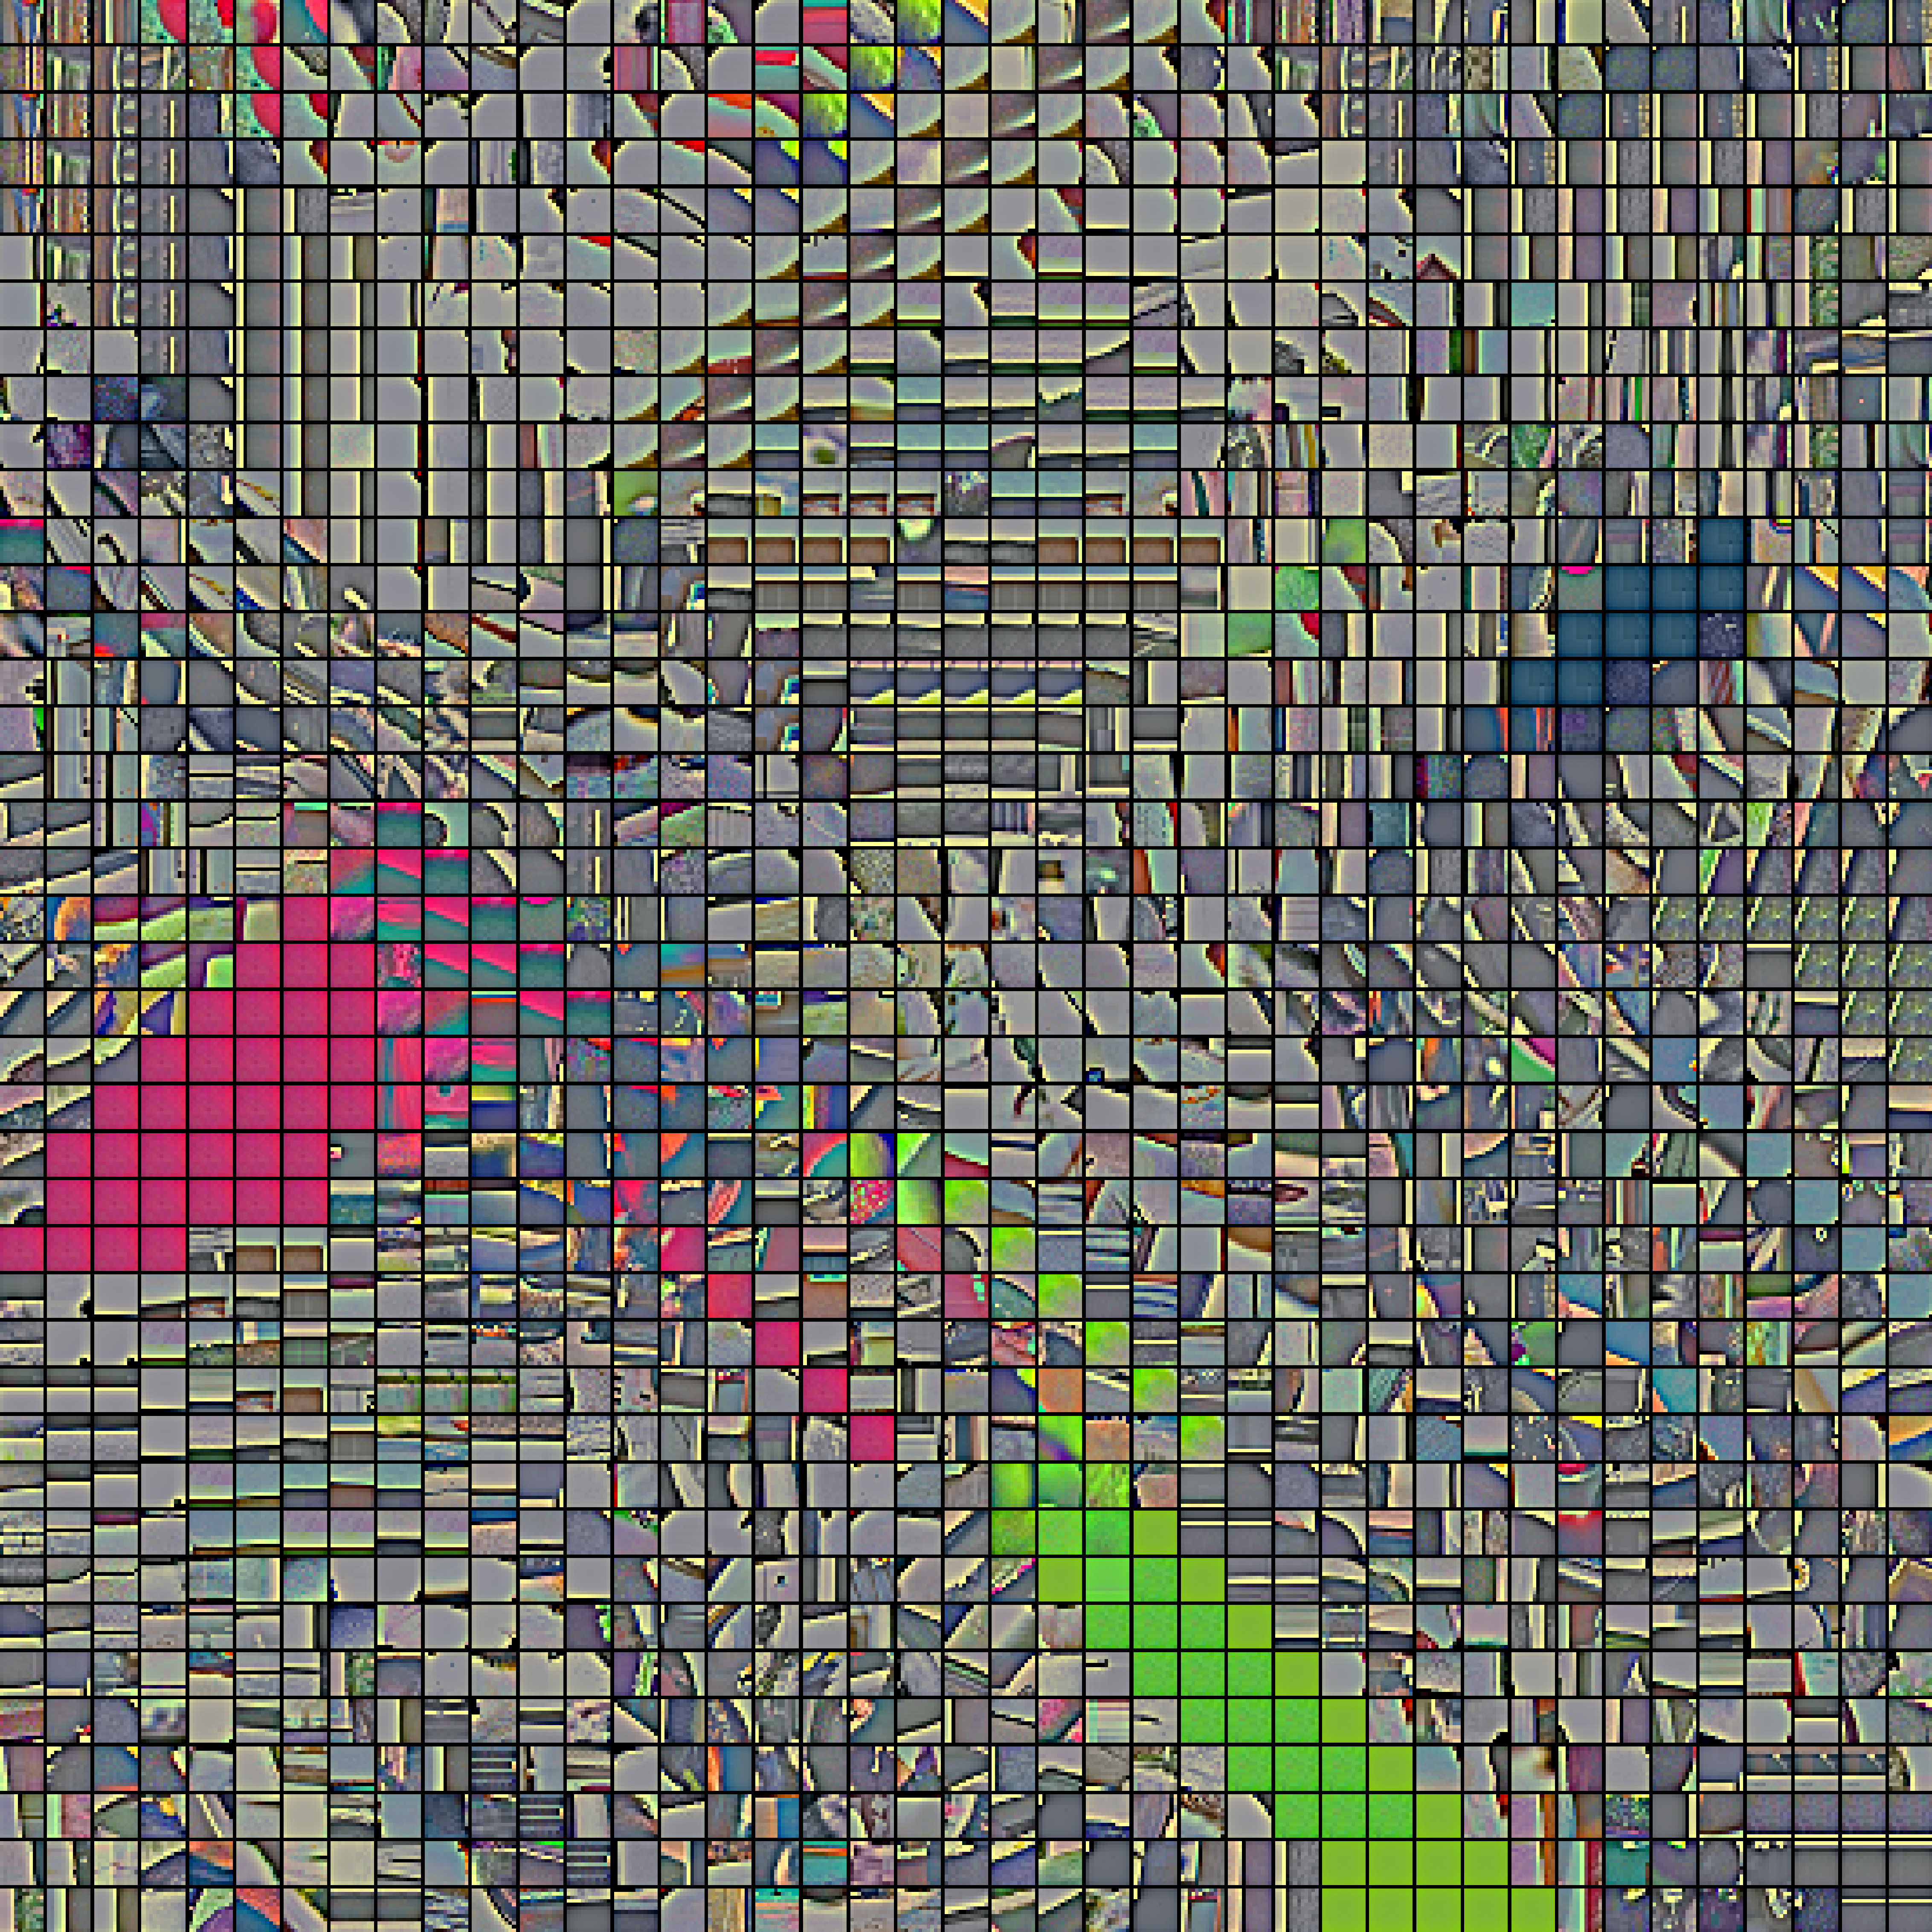
\includegraphics[width=0.28\linewidth]{figures/topographical_order_more_patches_imagenet128_patches_12}
  	  	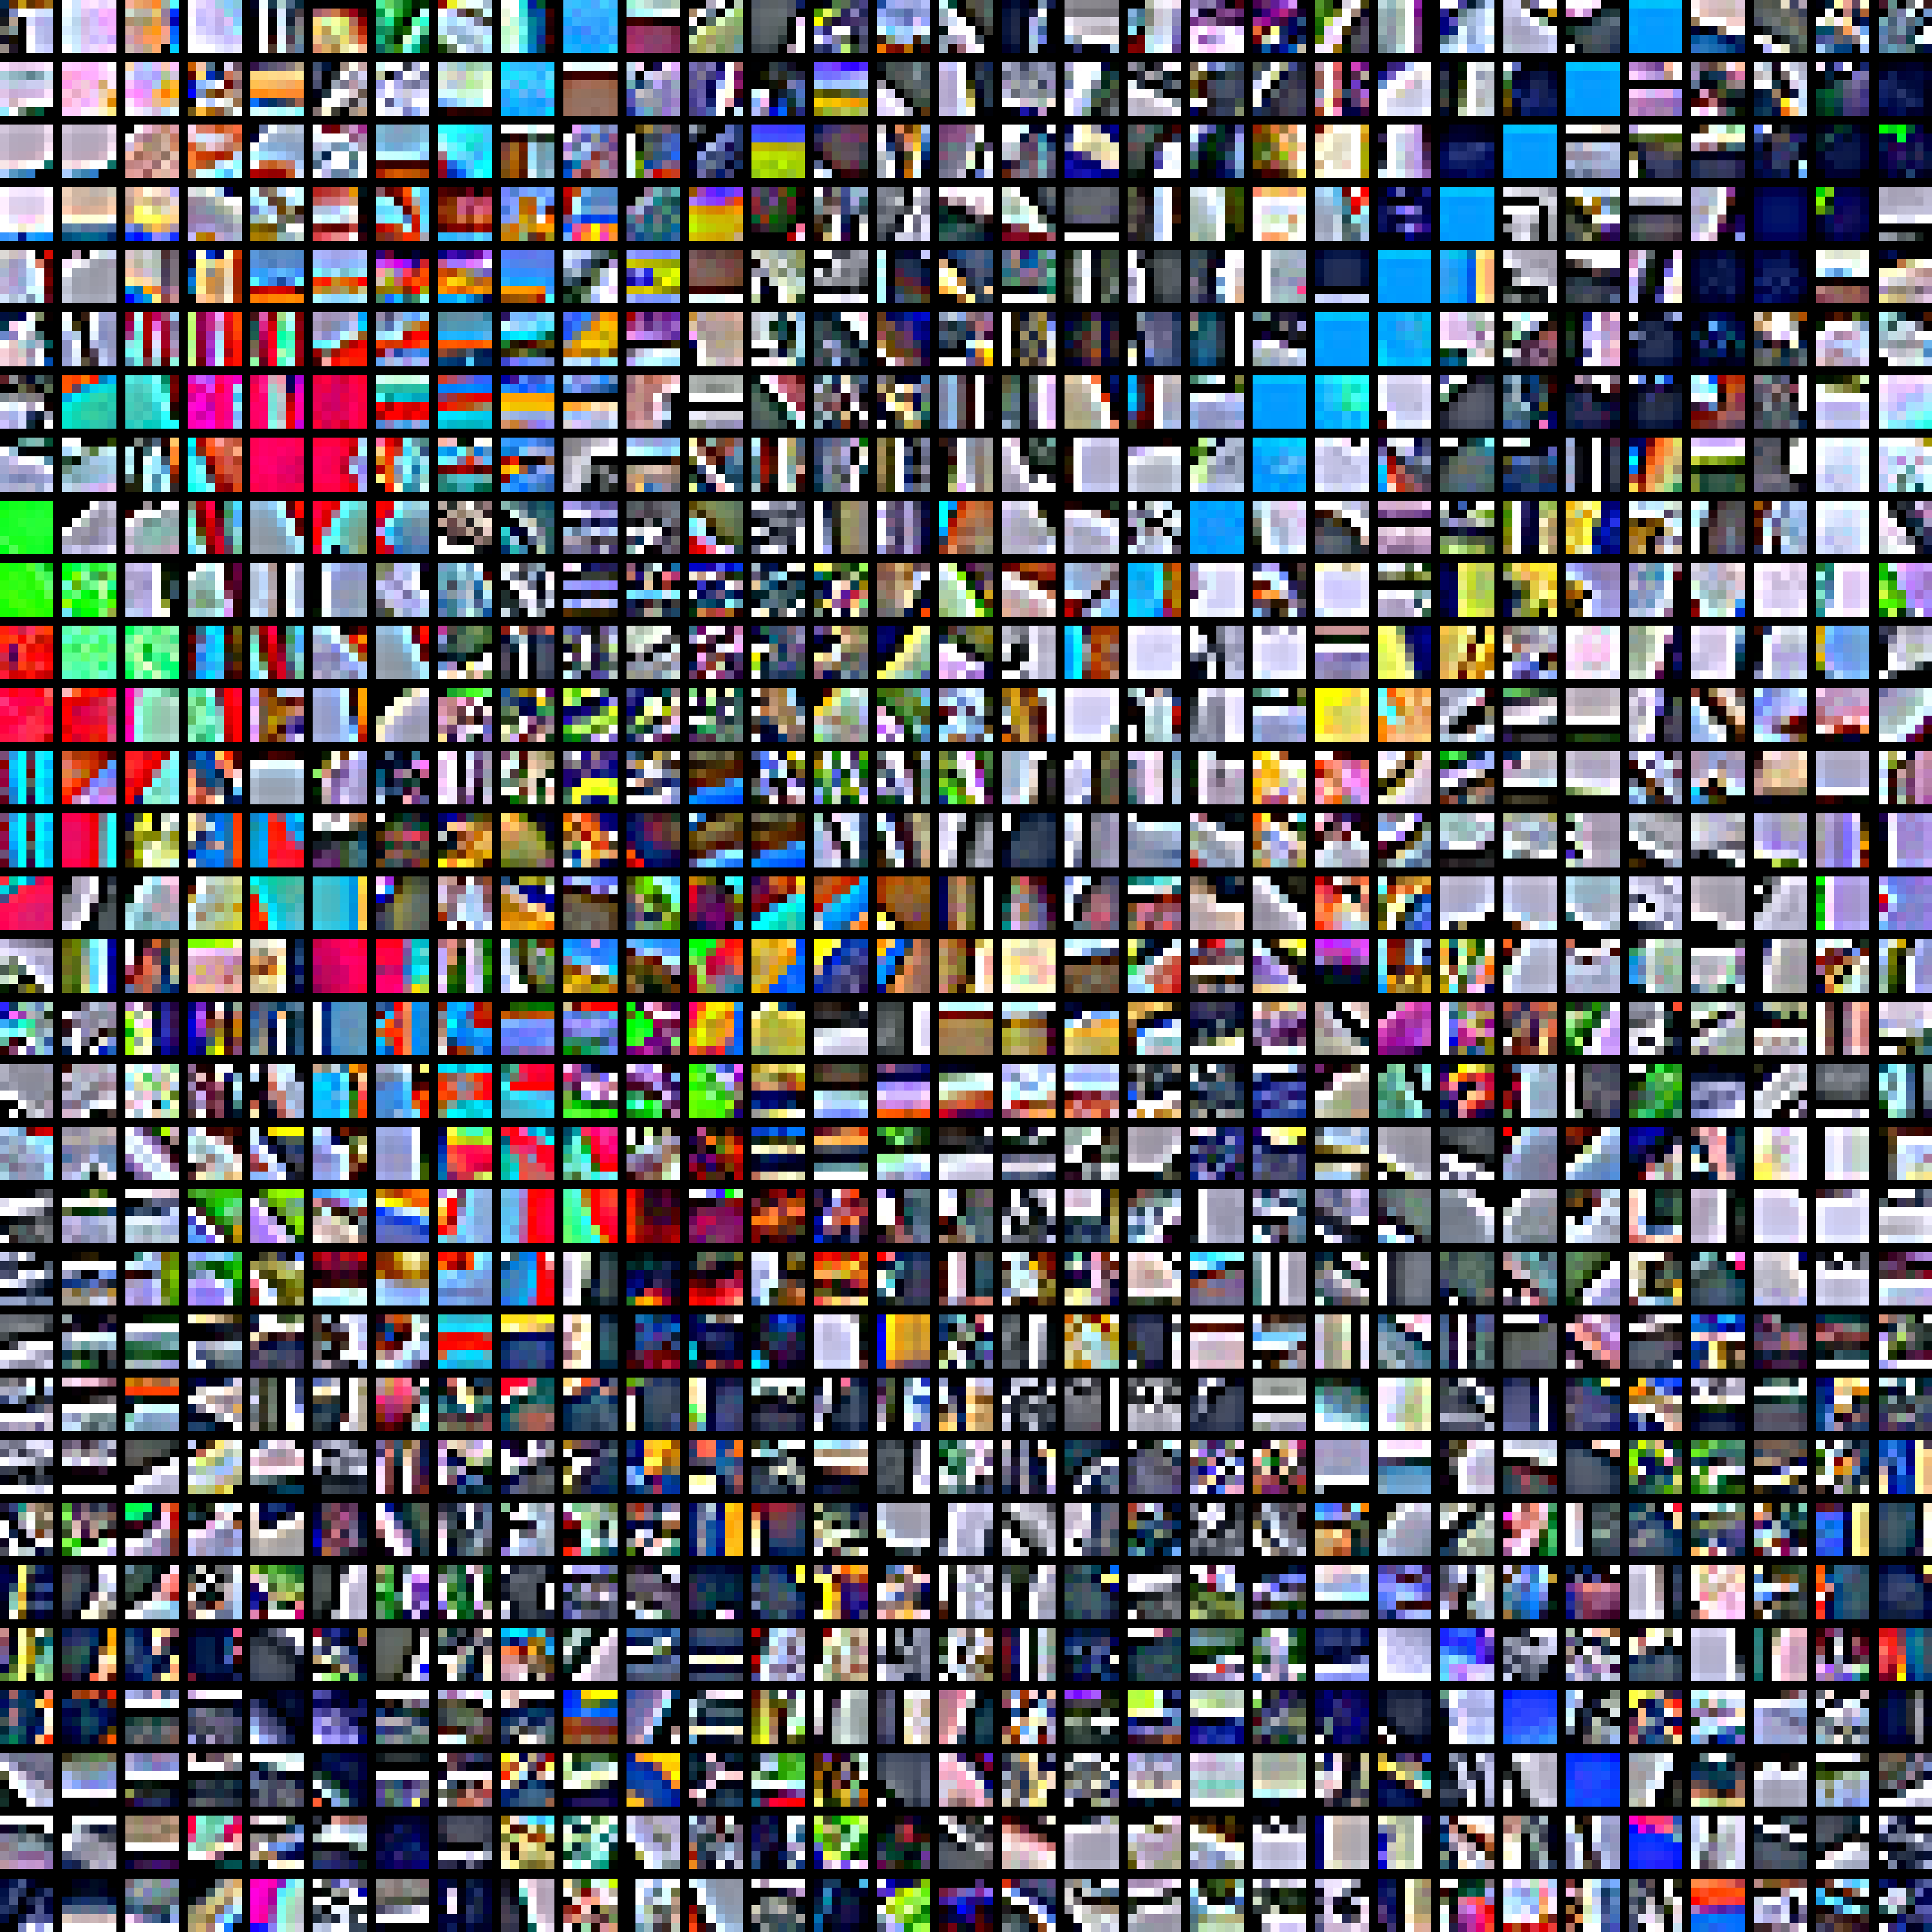
\includegraphics[width=0.28\linewidth]{figures/topographical_order_more_patches_imagnet64_patches_6_30Images}
  	  	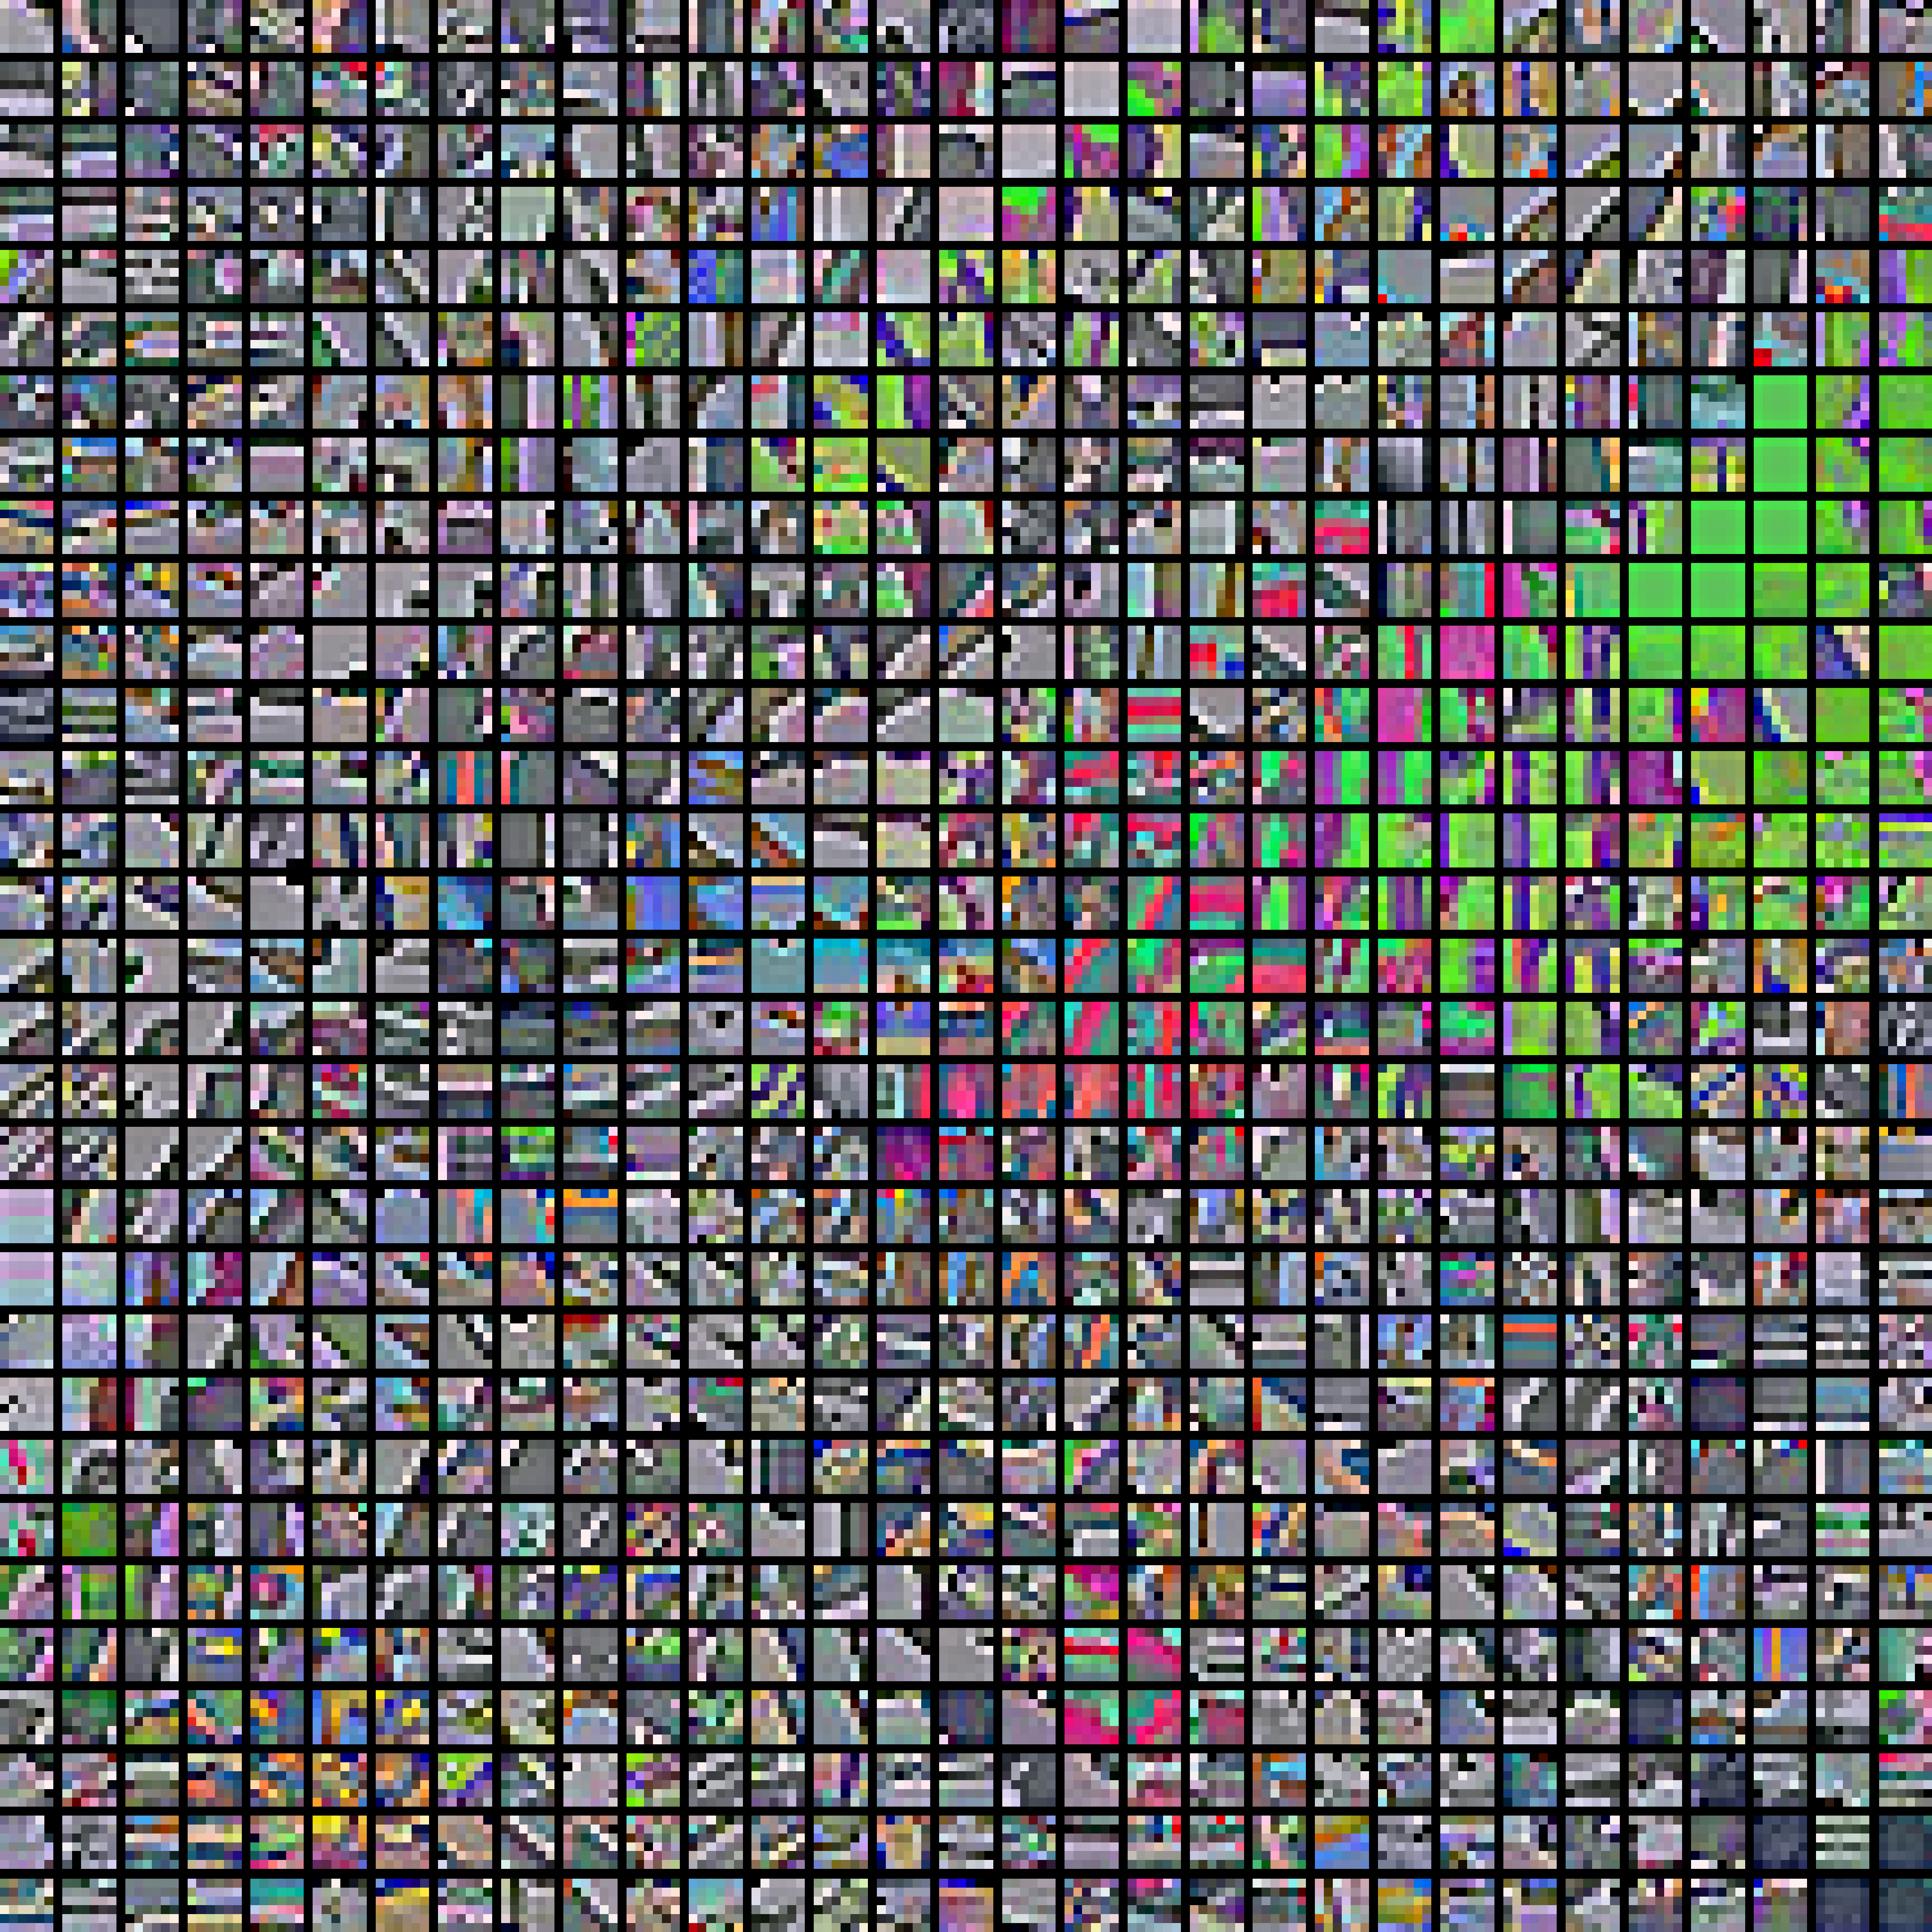
\includegraphics[width=0.28\linewidth]{figures/topographical_order_more_patches_cifar10_patches_6_30images}
\caption{An example of whitened dictionary  $\mathcal{D}$ with patch size $Q=6$ from ImageNet-128 (Left), ImageNet-64 (Middle), CIFAR-10 (Right). The atoms have been reordered via a topographic algorithm from \citet{Montobbio:2019} and contrast adjusted.}
\label{dico}
\end{figure}

\paragraph{$K$-Nearest Neighbors on patches}
The core idea of our algorithm is to compare the distances between each patch of an image and a fixed dictionary of patches $\mathcal{D}$, with size $|\mathcal{D}|$.
For a fixed dataset, this dictionary $\mathcal{D}$ is obtained by uniformly sampling patches from images over the whole training set. We augment $\mathcal{D}$ into $\cup_{d\in \mathcal{D}}\{d,-d\}$ because it allows the dictionary of patches to be contrast invariant and we observe it leads to better classification accuracies; we still refer to it as $\mathcal{D}$. An illustration is given by Fig.~\ref{dico}. Once the dictionary $\mathcal{D}$ is fixed, for each patch $p_{i,x}$ we consider the set $\mathcal{C}_{i, x}$ of pairwise distances $\mathcal{C}_{i, x} =\{\Vert p_{i, x} - d \Vert\,, d\in\mathcal{D} \} $.
For each whitened patch we encode the $K$-Nearest Neighbors of $p_{i,x}$ from the set $\mathcal{D}$, for some $ K \in \mathbb{N}$.
More formally, we consider $\tau_{i,x}$ the $K$-th smallest  element of $\mathcal{C}_{i,x}$, and we define the $K$-Nearest Neighbors binary encoding as follow, for $(d,i)\in\mathcal{D}\times\mathcal{I}$:
\begin{equation}
\label{encoding}
\phi(x)_{d,i}=
\begin{cases}
1,&\text{if } \Vert  p_{i,x} - d\Vert \leq \tau_{i,x}\\
0,&\text{otherwise}.
\end{cases} 
\end{equation}
Equation \ref{encoding} can be viewed as a Vector Quantization (VQ) step with hard-assignment \citep{coates2011importance}.
The representation $\phi$ encodes the patch neighborhood in a subset of randomly selected patches and can be seen as a crude description of the topological geometry of the image patches.
Moreover, it allows to view the distance between two images $x,y$ as a Hamming distance between the patches neighborhood encoding as:
\[\Vert \phi(x)-\phi(y)\Vert^2 = \sum_{i,d}\mathbf{1}_{\phi(x)_{d,i} \neq \phi(y)_{d,i}}\,.\]
In order to reduce the computational burden of our method, we perform an intermediary average-pooling step.
Indeed, we subdivide $\mathcal{I}$ in squared overlapping regions $\mathcal{I}_j\subset\mathcal{I}$, leading to the representation $\Phi$ defined, for $d\in\mathcal{D}, j$ by:
\begin{align}\Phi(x)_{d,j}= \sum_{i\in \mathcal{I}_j}\phi(x)_{d,i}\,.\end{align}
Hence, the resulting kernel is simply given by $K(x,y)= \langle \Phi(x),\Phi(y)\rangle $. Implementation details can be found in Appendix B. The next section describes our classification pipeline, as we feed our representation $\Phi$ to a linear classifier on challenging datasets.
%Note that due to the hard-assignment in VQ, it would not be possible to learn the parameters of our dictionary via a standard differentiable method, consequently this approach fails to be analyzed directly through the scope of \cite{chizat2018global} for instance.
\section{Experiments}
\label{experiments}
We train  shallow classifiers, i.e. linear classifier and 1-hidden layer CNN (1-CNN) on top of our representation $\Phi$ on two major  image classification datasets,  CIFAR-10 and ImageNet, which consist respectively of $5\times10^5$ small and $1.2\times10^6$ large color images  divided respectively into 10 and $10^3$ classes.
For training, we systematically used mini-batch SGD with momentum of 0.9, no weight decay and using the cross-entropy loss.


\paragraph{Classifier parametrization} In each experiments, the spatial subdivisions $\mathcal{I}_j$ are implemented as an average pooling with kernel size $k_1$ and stride $s_1$.
We then apply a 2D batch-normalization \citep{ioffe2015batch} in order to standardize our features on the fly before feeding them to a linear classifier.
In order to reduce the memory footprint of this linear classifier (following the same line of idea of a "bottleneck" \citep{he2016deep}), we factorize it into two convolutional operators.
The first one with kernel size $k_2$ and stride 1 reduces the number of channels from $\mathcal{D}$ to $c_2$ and the second one with kernel size $k_3$ and stride 1 outputs a number of channel equal to the number of image classes.
Then we apply a global average pooling.
For the 1-hidden layer experiment, we simply add a ReLU non linearity between the first and the second convolutional layer.




\subsection{CIFAR-10}
%\Edouard{E: wouldn't it be nice if we added an experiment with a gradient based representation, in order to show that a first order method doesn't learn more complex features than patches?}


%  \paragraph{Implementation details} For the linear classification experiments, we used an average pooling of size $k_1=5$ and stride $s_1=3$, $k_2=1$ and $c_2=128$ for the first convolutional operator and $k_3=6$ for the second one.
%  These values are set to  $k_1=3, s_1=2, k_2=3,c_2=2048, k_3=7$ for the 1-hidden layer experiments because they lead to better performances.
% Our data augmentation consists in horizontal random flips and random crops of size $32^2$ after reflect-padding with $4$ pixels. 
% For the dictionary, we choose a patch size of $Q=6$ and tested various sizes of the dictionary $|\mathcal{D}|$ and whitening regularization $\lambda=0.001$ . 
% In all cases, we used $K=0.4 |\mathcal{D}|$.%, which implies that our representation is not sparse.
% The model is trained for 175 epoch with a learning rate  decay 
% of 0.1 at epochs 100 and 150.
% The initial learning rate is $0.003$ for $|\mathcal{D}|=2.10^3$
% and $0.001$ for larger $|\mathcal{D}|$.
% \paragraph{Classification experiments} Our results are reported and compared in Tab.~\ref{cifar-acc}. First, note that contrary to experiments done by \cite{coates2011analysis} our methods has surprisingly good accuracy despite the hard-assignment in Vector Quantization.
% Sparse coding, soft-thresholding and orthogonal matching pursuit based representations used by \cite{coates2011importance, recht2019imagenet} can be seen as soft-assignment VQ and yield comparable classification accuracy (resp. 81.5\% with $6.10^3$ patches and 85.6\% with $2.10^5$ patches).
% However, these representations contain much more information than hard-assignment VQ as they allow to reconstruct a large part of the signal.
% Our representation yields better accuracy with only coarse topological information on the image patches, suggesting that this information is highly relevant for classification.
% To obtain comparable accuracies with a linear classifier, we use a single binary encoding step compared to \cite{mairal2016end} and we need a much smaller number of patches than \cite{recht2019imagenet, coates2011importance}.
% Moreover, \cite{recht2019imagenet} is the only work in the litterature, besides us, that achieves good performance using solely a linear model with depth one. 
% Using a 1-hidden layer classifier, our accuracy is competitive with deep kernel methods \citep{li2019enhanced,shankar2020neural} and deep supervised convolutional networks \citep{krizhevsky2012imagenet}.
% This further indicates the relevance of patches neighborhood information for classification task.
% %We also observe that using online optimization, in our case, didn't result in a drop in performance compared \citet{recht2019imagenet} where the linear regression is solved in closed form, suggesting the problem is well fairly well-conditionned. Furthermore, the performance doesn't seem to be sensitive to the choice of the loss (cross-entropy (ours) vs quadratic \citet{recht2019imagenet}  vs hinge \citet{mairal2016end}). 
% \begin{table}[h]
%   \caption{Accuracies on CIFAR-10\label{cifar-acc}. We compare methods relying on patch dictionaries. Q is the patch size, $|\mathcal{D}|$ the size of the patch dictionary, VQ indicates whether vector quantization with hard-assignment is applied and Classif. stands for classifier. 
%   %We observe that a linear classifier is sufficient to obtain high performance, demonstrated only with higher depth in other works. Compared to Recht et al our work shows that discarding information via hard-assignment VQ still allows to recover high performance. 
%   Amongst methods relying on random patches ours is the only approach operating online (and therefore allowing for scalable training). }
%   \label{accuracy}
%   \centering
%   \begin{tabular}{|c|c|c|c|c|c|c|c|}
%     \hline 
%     Method&$|\mathcal{D}|$&VQ&Online &$Q$&Depth &Classif.& Acc. \\
%     \hline 
%     SimplePatch (Ours)&$2\cdot10^3$ & \checkmark&\checkmark &6&1&linear&82.5 \\
%     \hdashline[0.5pt/1pt]
%     SimplePatch (Ours) &$1\cdot10^4$ & \checkmark&\checkmark & 6&1&linear&85.6\\
%     \hdashline[0.5pt/1pt]
%     SimplePatch (Ours) &$6\cdot10^4$ & \checkmark&\checkmark &6&1&linear&86.6\\
%     \hdashline[0.5pt/1pt]
%     \cite{coates2011analysis}&$1\cdot10^3$& \checkmark& $\times$&6 & 1&linear & 68.6\\\hdashline[0.5pt/1pt]
%   % \hline 
%     \cite{recht2019imagenet}&$2\cdot10^5$ & $\times$&$\times$&6&1&linear &85.6\\
%     \hdashline[0.5pt/1pt]
%     CKN \citep{mairal2016end}&$10^3, 10^4$& $\times$& $\times$&3 & 2& linear &85.8\\
%     \hdashline[0.5pt/1pt]
%     NK \citep{shankar2020neural}& - & $\times$& $\times$ &3&5&kernel &89.8\\
%     \hdashline[0.5pt/1pt]
%     NTK \citep{li2019enhanced}&$2 \cdot 10^3$& $\times$&$\times$ &6&6&kernel &88.9\\\hdashline[0.5pt/1pt]
%   SimplePatch (Ours)&$2\cdot10^3$ & \checkmark& \checkmark &6&2&1-CNN&88.5\\
%     \hline\hline
%   % \hdashline[0.5pt/1pt]
%     Scatt. \citep{Oyallon_2015_CVPR} & - & $\times$& $\times$&8 &2 & kernel & 82.3\\ \hdashline[0.5pt/1pt]
%     AlexNet \citep{krizhevsky2012imagenet}&-& $\times$& \checkmark &-&5&CNN&89.1\\
%     \hline
%   \end{tabular}
% \end{table}

%%% START MODIF
 \paragraph{Implementation details}
Our data augmentation consists in horizontal random flips and random crops of size $32^2$ after reflect-padding with $4$ pixels. 
For the dictionary, we choose a patch size of $Q=6$ and tested various sizes of the dictionary $|\mathcal{D}|$ and whitening regularization $\lambda=0.001$ . 
In all cases, we used $K=0.4 |\mathcal{D}|$.%, which implies that our representation is not sparse.
The classifier is trained for 175 epoch with a learning rate decay 
of 0.1 at epochs 100 and 150.
The initial learning rate is $0.003$ for $|\mathcal{D}|=2.10^3$
and $0.001$ for larger $|\mathcal{D}|$.

\paragraph{Linear classification experiments}  For the linear classification experiments, we used an average pooling of size $k_1=5$ and stride $s_1=3$, $k_2=1$ and $c_2=128$ for the first convolutional operator and $k_3=6$ for the second one.
Our results are reported and compared in Tab.~\ref{cifar-acc-linear}. First, note that contrary to experiments done by \cite{coates2011analysis} our methods has surprisingly good accuracy despite the hard-assignment in Vector Quantization.
Sparse coding, soft-thresholding and orthogonal matching pursuit based representations used by \cite{coates2011importance, recht2019imagenet} can be seen as soft-assignment VQ and yield comparable classification accuracy (resp. 81.5\% with $6.10^3$ patches and 85.6\% with $2.10^5$ patches).
However, these representations contain much more information than hard-assignment VQ as they allow to reconstruct a large part of the signal.
Our representation yields better accuracy with only coarse topological information on the image patches, suggesting that this information is highly relevant for classification.
To obtain comparable accuracies with a linear classifier, we use a single binary encoding step compared to \cite{mairal2016end} and we need a much smaller number of patches than \cite{recht2019imagenet, coates2011importance}.
Moreover, \cite{recht2019imagenet} is the only work in the litterature, besides us, that achieves good performance using solely a linear model with depth one.
To test the VQ importance, we replace the hard-assignment VQ implemented with a binary non-linearity  $\mathbf{1}_{\Vert  p_{i,x} - d\Vert \leq \tau_{i,x}}$ (see Eq. \ref{encoding}) by a soft-assignment VQ with a sigmoid function $(1 + e^{\Vert  p_{i,x} - d\Vert - \tau_{i,x}})^{-1}$.
The accuracy increases by $0.2\%$, showing that the use soft-assignment in VQ which is crucial for performance in \cite{coates2011importance} does not affect much the performances of our representation.

\begin{table}[h]
  \caption{One layer patch-based classification accuracies on CIFAR-10\label{cifar-acc-linear}. We compare methods relying on patch dictionaries. Q is the patch size, $|\mathcal{D}|$ the size of the patch dictionary, VQ indicates whether vector quantization with hard-assignment is applied. 
  %We observe that a linear classifier is sufficient to obtain high performance, demonstrated only with higher depth in other works. Compared to Recht et al our work shows that discarding information via hard-assignment VQ still allows to recover high performance. 
  Amongst methods relying on random patches ours is the only approach operating online (and therefore allowing for scalable training). }
  \label{accuracy}
  \centering
  \begin{tabular}{|c|c|c|c|c|c|c|}
    \hline 
    Method&$|\mathcal{D}|$&VQ&Online &$Q$ & Acc. \\
    \hline 
    % SimplePatch (Ours)&$2\cdot10^3$ & \checkmark&\checkmark &6&1&82.5 \\
    % \hdashline[0.5pt/1pt]
    SimplePatch (Ours) &$1\cdot10^4$ & \checkmark&\checkmark & 6&85.6\\
    \hdashline[0.5pt/1pt]
    SimplePatch (Ours) &$6\cdot10^4$ & \checkmark&\checkmark &6&86.7\\
    \hdashline[0.5pt/1pt]
    SimplePatch (Ours) &$6\cdot10^4$ & $\times$&\checkmark &6&\textbf{86.9}\\
    \hdashline[0.5pt/1pt]
     \cite{ba2014deep}&$4\cdot10^3$&$\times$&\checkmark&-&81.6\\
    \hdashline[0.5pt/1pt]
    \cite{coates2011analysis}&$1\cdot10^3$& \checkmark& $\times$&6 & 68.6\\
        \hdashline[0.5pt/1pt]
    Scatt. \citep{Oyallon_2015_CVPR} & - &$\times$& $\times$& 8 &  82.2\\
    \hdashline[0.5pt/1pt]
   % \hline 
    \cite{recht2019imagenet}&$2\cdot10^5$ & $\times$&$\times$&6&85.6\\
    \hline
  \end{tabular}
\end{table}


\paragraph{Importance of data-driven representations}
% As observed by some  works from Tab.~\ref{cifar-acc-linear} and ~\ref{cifar-acc-non-linear}, removing the whitening step for both the dictionary and image patches leads to  a  performance drop  of about 17\%.
As we see in Tab. ~\ref{cifar-acc-data-driven}, the data-driven representation is crucial for good performance of handcrafted kernel classifiers.
In our setting, removing the patches whitening and replacing the whitened dictionary of patches by samples from a white Gaussian distribution and  step leads to a drop of  8.1 \% . \Edouard{Comparison with a trained end-to-end SimplePatch? I bet it'll do worse!}


\paragraph{Non-linear classification experiments}
As a non linear classifier, we simply use 1-hidden layer classifier with ReLU non linearity using an average pooling of size $k_1=3$ and stride $s_1=2$, $k_2=3$, $c_2=2048$ and $k_3=7$ .
Our results are reported and compared with other non-linear classification methods in Tab.~\ref{cifar-acc-non-linear}.
With this 1-hidden layer classifier, our accuracy is competitive with deep kernel methods \citep{li2019enhanced,shankar2020neural} and deep supervised convolutional networks \citep{krizhevsky2012imagenet}.
This further indicates the relevance of patches neighborhood information for classification task.
%We also observe that using online optimization, in our case, didn't result in a drop in performance compared \citet{recht2019imagenet} where the linear regression is solved in closed form, suggesting the problem is well fairly well-conditionned. Furthermore, the performance doesn't seem to be sensitive to the choice of the loss (cross-entropy (ours) vs quadratic \citet{recht2019imagenet}  vs hinge \citet{mairal2016end}). 
\begin{table}[h]
  \caption{Accuracies on CIFAR-10 with Handcrafted Kernels classifiers with and without data-driven reprensentations \label{cifar-acc-data-driven}. For SimplePatch we replace patches with random gaussian noise. \Edouard{RAJOUTER: https://arxiv.org/abs/2006.13645 ?}
  }
  \label{accuracy}
  \centering
  \begin{tabular}{|c|c|c|c|c|c|c|c|}
    \hline 
    Method&VQ&Online &Depth & Accuracy & \small Data used &Improvement \\
    &&&&(\textbf{not} data driven && \small (data driven)    \\
    \hline
        Simple (random) Patch (Ours) & \checkmark & \checkmark & 1 &78.6 & Patches & 8.1 \\
    \hdashline[0.5pt/1pt]
    NK \citep{shankar2020neural} & $\times$& $\times$ &5 &77.7&ZCA&8.1\\
    \hdashline[0.5pt/1pt]
    CKN \citep{mairal2016end}&$\times$& $\times$&2&81.1&Patches&5.1\\%85.8
    \hdashline[0.5pt/1pt]
    NTK \citep{li2019enhanced}&$\times$& $\times$&8 &82.2&Patches&6.7\\
    \hdashline[0.5pt/1pt]
    Linearized\citep{samarin2020empirical}&$\times$& $\times$&\Edouard{??}&65.6 &e2e&13.2\\
     %&88.9\\
    \hline
  \end{tabular}
\end{table}



\begin{table}[h]
  \caption{Accuracies on CIFAR-10 with shallow supervised classifiers \label{cifar-acc-non-linear}. We compare methods relying on patch dictionaries. Q is the patch size, $|\mathcal{D}|$ the size of the patch dictionary, VQ indicates whether vector quantization with hard-assignment is applied and Classif. stands for classifier. 
  %We observe that a linear classifier is sufficient to obtain high performance, demonstrated only with higher depth in other works. Compared to Recht et al our work shows that discarding information via hard-assignment VQ still allows to recover high performance. 
  Amongst methods relying on random patches ours is the only approach operating online (and therefore allowing for scalable training). }
  \label{accuracy}
  \centering
  \begin{tabular}{|c|c|c|c|c|c|}
    \hline 
    Method&VQ (1st layer)&Depth &Classif.& Acc. \\
    \hline
     SimplePatch (Ours) & \checkmark &2&1-layer&88.5\\
    \hdashline[0.5pt/1pt]
    NK \citep{shankar2020neural} & $\times$ &5&e2e &89.8\\
    \hdashline[0.5pt/1pt]
    CKN \citep{mairal2016end}& $\times$ & 9&e2e& 89.8\\
    \hdashline[0.5pt/1pt]
    AlexNet \citep{krizhevsky2012imagenet}& $\times$ &5&e2e&89.1\\
    \hline
  \end{tabular}
\end{table}








%%% END MODIF

\begin{figure} 
    \centering
    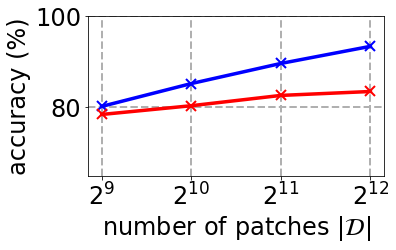
\includegraphics[width=0.245\linewidth]{figures/ablation_npatches.png}
    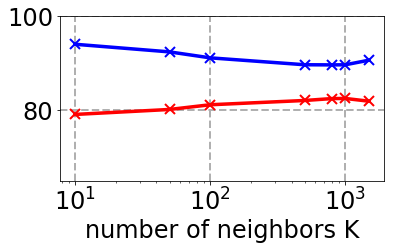
\includegraphics[width=0.245\linewidth]{figures/ablation_K.png}
    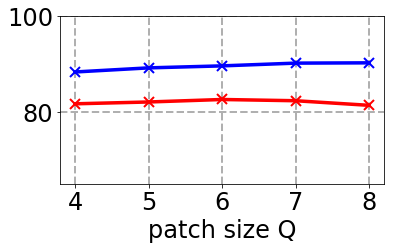
\includegraphics[width=0.245\linewidth]{figures/ablation_Q.png}
    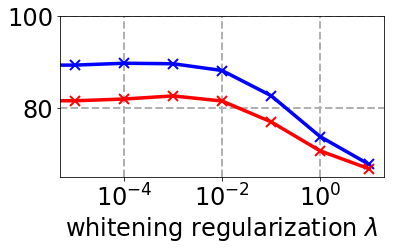
\includegraphics[width=0.245\linewidth]{figures/ablation_lambda.png}\\
    \caption{
        CIFAR-10 ablation experiments, train accuracies in blue, test accuracies in red. Higher resolution plots can be found in  Appendix C.}
    \label{fig:ablation_study}
\end{figure}

\paragraph{Ablation experiments}
CIFAR-10 is a relatively small dataset that allows fast benchmarking, thus we conducted several ablation experiments in order to understand the relative improvement due to each hyper-parameter of our pipeline. We thus vary the size of the dictionary $|\mathcal{D}|$, the patch size $Q$, the number of nearest neighbors $K$ and the whitening regularization $\lambda$ which are the hyper-parameters of $\Phi$. Results are shown in Fig. \ref{fig:ablation_study}.


% \Edouard{\sout{
% Note that our representation is absolutely not sparse.The number of patches $|\mathcal{D}|$ varies in $\lbrace 512, 1024, 2048, 4096 \rbrace$, the patch size $Q$ varies in $\lbrace 4, 5, 6, 7, 8 \rbrace$, the number of neighbors $K=
% $ varies in $\lbrace 10, 50, 100, 500, 800, 1000, 1500 \rbrace$ and  the whitening regularizer $\lambda$ varies in $\lbrace0, 10^{-5}, 10^{-4}, 10^{-3}, 10^{-2}, 10^{-1}, 1, 10\rbrace$.
% Results are shown in figure \ref{fig:ablation_study}.}}

Note that even a relatively small number of patches is competitive with much more complicated representations, such as \citet{Oyallon_2015_CVPR}.
While it is possible to slightly optimize the performances according to $K$ or $Q$,  the fluctuations remain minor compared to other factors, which indicate that the performances of our method are relatively stable w.r.t. this set of hyper-parameters. The whitening regularization behaves similarly to a thresholding operator on the eigenvalues of $\Sigma^{1/2}$: the larger it is, the more it penalizes larger eigenvalues. Interestingly, we note that under a certain threshold, this hyper-parameter  does almost not affect the classification performances. This goes in hand with both a fast eigenvalue decay and a stability to noise, that we discuss further in Sec. \ref{structure}.

% \paragraph{Classifier factorization}
% In order to test the inductive bias of our classifier, we  replace it with a simple fully connected layer, with $6$ times more parameters than ours: the train and test accuracies are $93.0\%$ and $81.6\%$ compared to $88.9\%$ and $82.5\%$. The use of this factorized classifier significantly reduces overfitting, while reducing the number of computations. We note that using convolutions is well motivated by the  structure of natural images whose class is relatively invariant to translation.



\subsection{ImageNet}

% \paragraph{Implementation details}  Since ImageNet is a much larger dataset than CIFAR-10, we could  use no more than $|\mathcal{D}|=2048$ patches.
% Here, $\lambda=10^{-2}, k_1=5,s_1=3, k_2=1, c_2=256, k_3=12, Q=6$. For the 1-hidden layer experiment, we used $k_2=3$.
% In order to reduce the computational overhead of our method on ImageNet, we followed the same approach as \cite{DBLP:journals/corr/ChrabaszczLH17}. We reduce the resolution to $64^2$ as in \cite{DBLP:journals/corr/ChrabaszczLH17}, instead of the standard 224 length.  Note that \cite{DBLP:journals/corr/ChrabaszczLH17}  observed that this does not alterate much the top-performances of standard models ($5 \%$ to $10\%$ drop of accuracy on average), and we also believe it introduces a useful dimensionality reduction, as it removes high-frequency part of images that are  unstable
% \citet{mallat1999wavelet}.
% To measure the importance of the resolution on the performances, we also run a linear classification experiment on  ImageNet images with resolution $128^2$ using the same hyper-parameters except that we double the resolution of the initial operator (i.e., $Q=12, k_1=10,s_1=6$).
% Our models are trained during 60 epochs with an initial learning rate of 0.003 decayed by a factor 10 at epochs 40 and 50.
% During training, similarly to \cite{DBLP:journals/corr/ChrabaszczLH17} we use random flip and we select random crops of size of size $64^2$ , after a reflect-padding of size 8. At testing, we simply resize the image to $64^2$.


\paragraph{Implementation details} 
To reduce the computational overhead of our method on ImageNet, we followed the same approach as \cite{DBLP:journals/corr/ChrabaszczLH17}. We reduce the resolution to $64^2$ as in \cite{DBLP:journals/corr/ChrabaszczLH17}, instead of the standard 224 length.  Note that \cite{DBLP:journals/corr/ChrabaszczLH17}  observed that this does not alter much the top-performances of standard models ($5 \%$ to $10\%$ drop of accuracy on average), and we also believe it introduces a useful dimensionality reduction, as it removes high-frequency part of images that are  unstable
\citep{mallat1999wavelet}. 
We set the patch size to $Q=6$ and the whitening regularization to $\lambda=10^{-2}$. 
Since ImageNet is a much larger dataset than CIFAR-10, we restricted to $|\mathcal{D}|=2048$ patches. As for CIFAR-10 experiments, we set $K=0.4 |\mathcal{D}|$. The parameters of the linear convolutional classifier are chosen to be: $k_1=5,s_1=3,k_2=1, c_2=256, k_3=12$. For the 1-hidden layer experiment, we used kernel size of $k_2=3$ for the first convolution.
Our models are trained during 60 epochs with an initial learning rate of 0.003 decayed by a factor 10 at epochs 40 and 50.
During training, similarly to \cite{DBLP:journals/corr/ChrabaszczLH17} we use random flip and we select random crops of size $64$, after a reflect-padding of size 8. At testing, we simply resize the image to $64$.
Note that this procedure differs slightly from the usual data-augmentation, which consists in resizing images while maintaining ratios, before a random cropping.


\paragraph{Classification experiments}
Tab.~\ref{imagenet-xp} reports the accuracy of our method, as well as the accuracy of comparable methods. Using a smaller resolution for the images still allows our method to outperform by a large margin ( about $\sim 10\%$ Top-5) the  Scattering Transform \citep{mallat2012group}, which was the previous state-of-the-art-method in the context of no-representation learning.
% Note that it also outperforms randomly initialized neural networks \citep{arandjelovic2017look}.
Note that our representation uses only $2.10^3$ randomly selected patches which is a tiny fraction of the billions of ImageNet patches.

% \cite{sanchez2013image} obtain $72.0\%$ top-5 accuracy with a patch representation computed in three steps (SIFT, Fisher kernel, power-normalization/compression) and of dimension $6.10^4$.
% Using a representation of dimension $4.10^3$ they obtain $64.1\%$ top-5 accuracy.
% The performance of our method tested on lower resolution images ($128^2$) using a representation of dimension $2.10^3$ ($=|\mathcal{D}|$) is relatively close to the performance of the $4.10^3$ dimensional Fisher Vectors, but further large scale experiments would be needed to confirm if this holds for higher dimensions.
% Note that this visual representation involves the learning of a Gaussian mixture model and several PCA dimensionality reductions that are crucial for performance.
%Still, a major difference between our representation and both Scattering Transform and Fisher Vector is the hard-assignment VQ that discards signal information while the image can be fairly reconstructed using Scattering coefficients \citep{oyallon2017scaling} or SIFT descriptors \citep{weinzaepfel2011reconstructing}.

We now compare our performances with supervised models trained end-to-end.
BagNets \citep{brendel2019approximating} have shown that  competitive classification accuracies can be obtained with patch-encoding that consists of 50 layers.
The performance obtained by our shallow experiment with a 1-hidden layer classifier reduces significantly the gap of performance between our method and a BagNet with similar patch-size.
This suggests once again that hard-assignment VQ does not degrade much of the classification information.
We also note that our approach with a linear classifier outperforms supervised shallow baselines that consists of 1 or 2 hidden-layers CNN \citep{belilovsky2018greedy}, which indicates that a patch based representation is a non-trivial baseline.

To measure the importance of the resolution on the performances, we run a linear classification experiment on ImageNet images with twice bigger resolution ($128^2$ images , $Q=12, k_1=10,s_1=6$).
We observe that it improves classification performances.
Note that the patches used are in a space of dimension $432 \gg 1$: this improvement is surprising since distance to nearest neighbors are known to be meaningless in high-dimension \citep{beyer1999nearest}.
This shows a form of low-dimensionality in the natural image patches, that we study in the next Section.

%\paragraph{Random filters and whitening} On Imagenet64, removing the whitening step leads to an accuracy of $18\%$ top-1, i.e. a drop of about 16\%. Like for CIFAR-10, this step is crucial for performance.
\begin{table}[h]
  \caption{Handcrafted kernel accuracies on ImageNet, where no ad-hoc explicit loss is optimized. D., Res. and Classif. stand respectively for Depth, Resolution and  Classifier.
  Dim. stands for the dimension of the patch representation equal to $|\mathcal{D}|$ in our setting. \Edouard{more results???}
  \label{imagenet-xp}}
  \label{accuracy}
  \centering
  \begin{tabular}{|c|c|c|c|c|c|c|c|c|}
    \hline 
    Method &  Dim. &VQ & $Q$ & D. & Res. & Classif. & Top1 & Top5 \\
    \hline 
    \hline
    SimplePatch(Ours)&$2.10^3$& \checkmark &  6 & 1 & 64 & linear & 33.4 &  54.7 \\
    \hdashline[0.5pt/1pt]
    SimplePatch(Ours)&$2.10^3$ & \checkmark & 12 & 1 & 128 & linear & 35.4  &  56.9 \\
    \hdashline[0.5pt/1pt]
    SimplePatch(Ours)&$2.10^3$ & $\times$ & 12 & 1 & 128 & linear & 35.8  &  \textbf{57.1} \\
    \hdashline[0.5pt/1pt]
    Scatt.\citep{zarka2019deep} & -& $\times$& 32 & 2 & 224 & linear & 26.1  & 44.7 \\
    \hdashline[0.5pt/1pt]
    Random\citep{arandjelovic2017look} &- &$\times$& - &9 & 224 & linear & 18.9  & -\\
    \hdashline[0.5pt/1pt]
    AlexLinearized \citep{samarin2020empirical}&-&$\times$&-&9&224&\text{linear}&\Edouard{??}&39.2\\
    %\hline
    %Fisher Vector\citep{sanchez2013image} &  \checkmark &$4. 10^3$ &$\times$& 24 & 3 & full& linear & - & 64.1\\
    %\hdashline[0.5pt/1pt]
    %Fisher Vector\citep{sanchez2013image} & \checkmark & $6. 10^4$ &$\times$& 24 & 3 & full& linear & - & 72.0\\
    \hline
  \end{tabular}
\end{table}


\begin{table}[h]
  \caption{Supervised accuracies on ImageNet. D., Res. and Classif. stand respectively for Depth, Resolution and  Classifier.
  Dim. stands for the dimension of the patch representation equal to $|\mathcal{D}|$ in our setting.
  \label{imagenet-xp}}
  \label{accuracy}
  \centering
  \begin{tabular}{|c|c|c|c|c|c|c|c|c|}
    \hline 
    Method &  Dim. &VQ & $Q$ & D. & Res. & Classif. & Top1&Top5 \\
    \hline 
    \hline
     SimplePatch(Ours)& $2.10^3$ & \checkmark & 6 & 2 & 64 & 1-layer & 39.4 &  62.1 \\
     \hdashline[0.5pt/1pt]
   Shallow\citep{belilovsky2018greedy}&-&$\times$&-&1&224&e2e&-&26\\
    \hdashline[0.5pt/1pt]
   Shallow\citep{belilovsky2018greedy}&-&$\times$&-&2&224&e2e&-&44\\
   \hdashline[0.5pt/1pt]
   BagNet\citep{brendel2019approximating}  & - &$\times$& 9 & 50 & 224 & e2e & - & 70.0\\
    %\hdashline[0.5pt/1pt]
    %AlexNet\citep{krizhevsky2012imagenet}& -&$\times$&-&10&224&CNN&56.5&79.1\\
   \hline
  \end{tabular}
\end{table}

\begin{figure}[h]
    \centering
    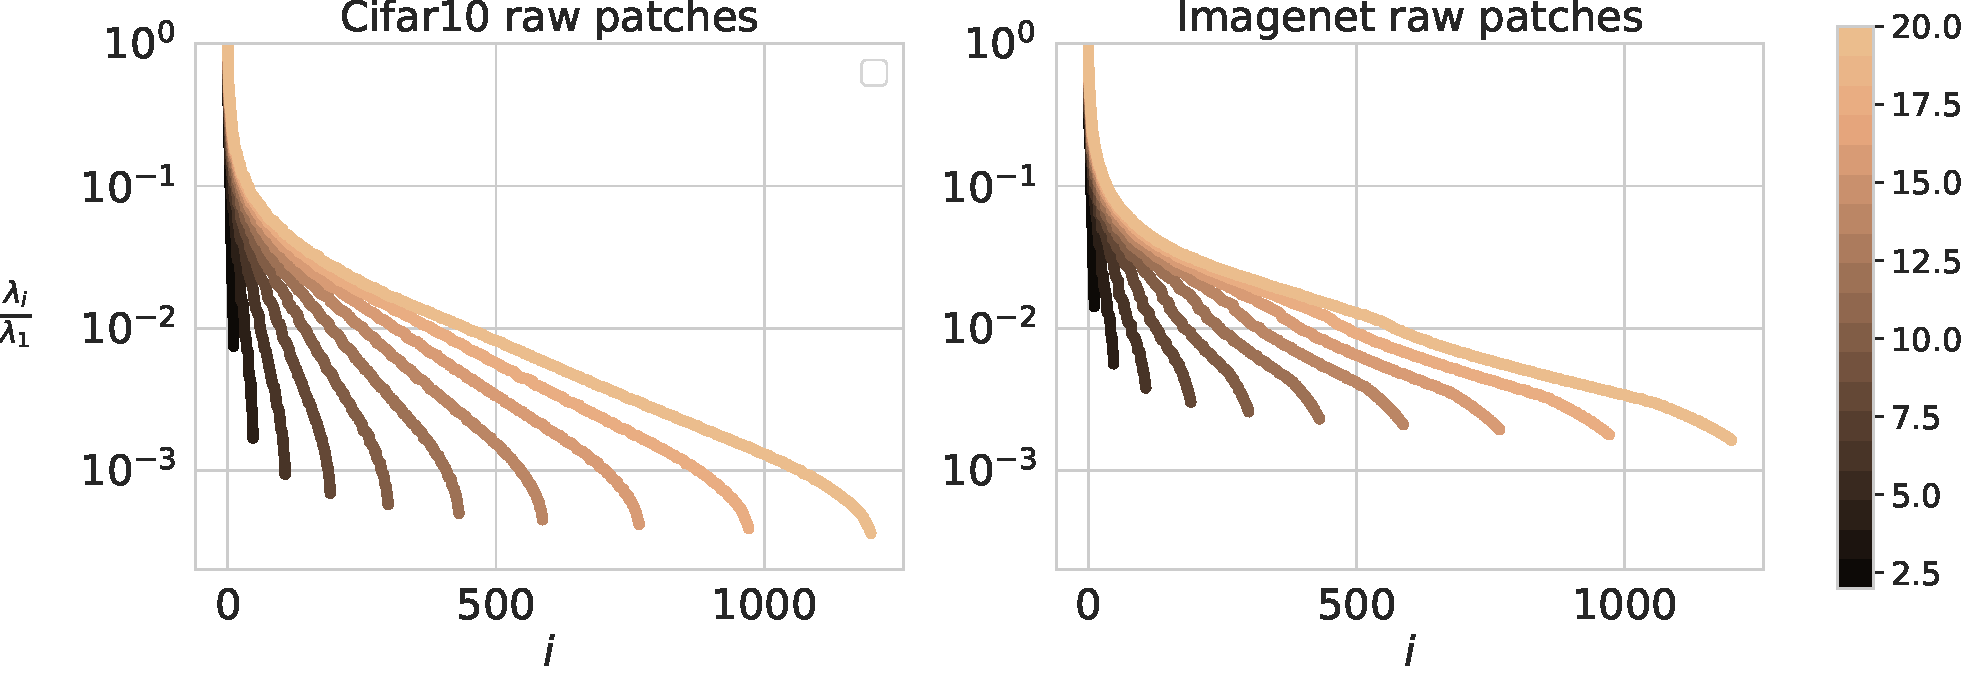
\includegraphics[width=.9\linewidth]{figures/spectrum_patches}
	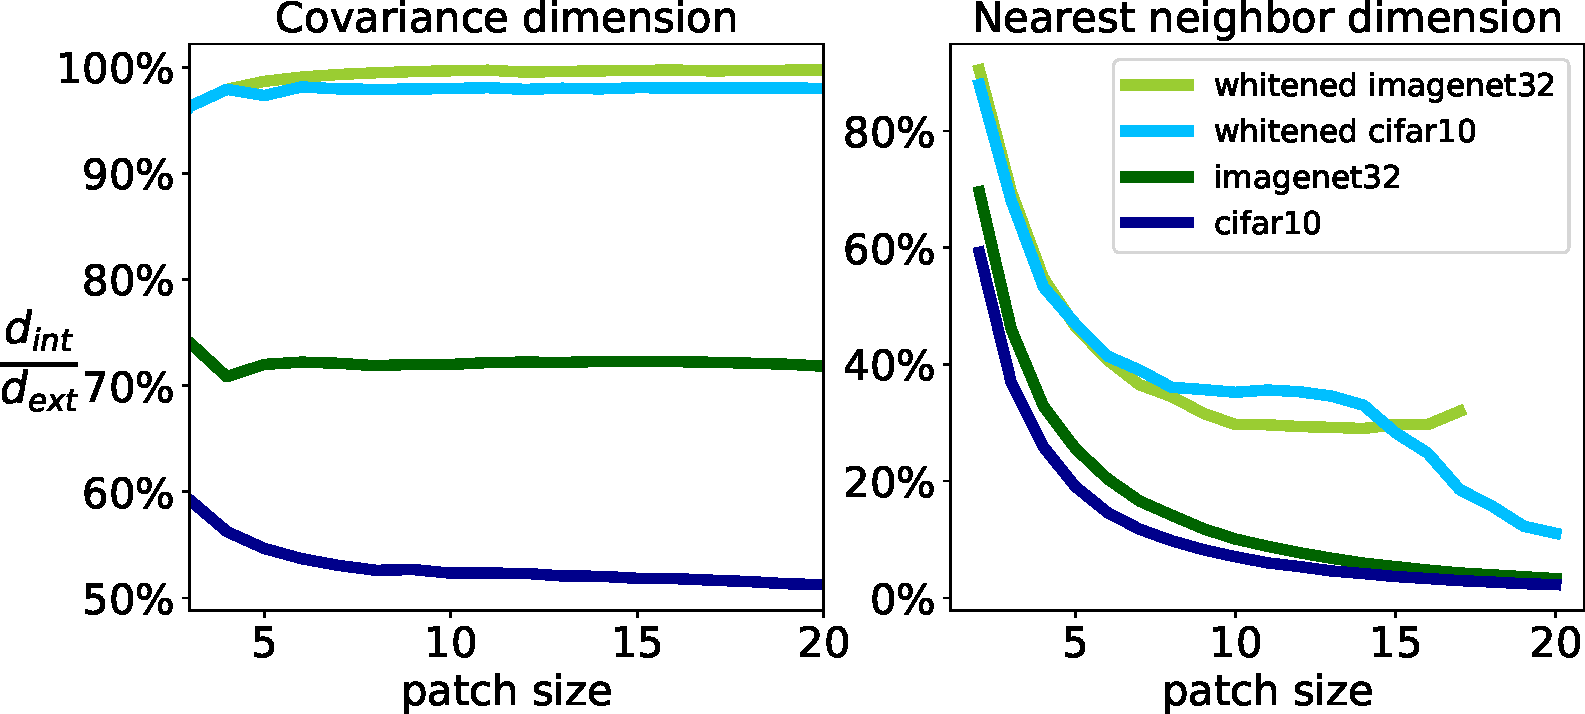
\includegraphics[width=.9\linewidth]{figures/intrinsic_dims}
	\caption{(Top) Spectrum  of the square root covariance matrix $\Sigma^{1/2}$ on CIFAR-10 (top-left) and ImageNet-64 (top-right) using small patch sizes in dark-brown to larger patch sizes in light-brown.\\
	(Bottom-left) Covariance dimension as a function of the extrinsic dimension of the patches and (bottom right) nearest neighbor dimension as a functions of the extrinsic dimension of the patches.}
	\label{fig:spec_intrinsic_dim}
\end{figure}


\subsection{Dictionary structure}
\label{structure}

\paragraph{Spectrum of $\mathcal{D}$}
Fig. \ref{fig:spec_intrinsic_dim} (top) shows the spectrum of $\Sigma^{1/2}$ for  several values of $Q$, normalized by $\Vert \Sigma^{1/2}\Vert$ on CIFAR-10 and ImageNet-32.  First, note that the spectrum tends to decay at an exponential rate (linear rate in semi-logarithmic scale). This rate decreases as the size of the patch increases (from dark brown to light brown) suggesting an increased linear dimensionality for larger patches. The second observation is that patches from ImageNet-32 dataset tend to be better conditioned than those from CIFAR-10 with a conditioning ratio of $10^2$ for ImageNet vs $10^3$ for CIFAR-10. This is probably due to the use of more diverse images than on CIFAR-10. From this spectrum, it is straightforward to compute the linear dimensionality of the patches. Fig.
~\ref{fig:spec_intrinsic_dim}(bottom-left) shows the number of axis needed to explain $95\%$ of the variance as a function of the extrinsic dimension $d_{\rm ext} = 3Q^2$, with and without whitening. Before whitening, this linear dimension is much smaller than the ambient dimension: whitening the patches increases the linear dimensionality of the patches, which still increases at a linear growth as a function of $Q^2$.


\paragraph{Intrinsic dimension of $\mathcal{D}$}
We propose to refine our measure of linear dimensionality to a non-linear measure of the intrinsic dimension. Indeed, under the assumption of low-dimensional manifold, the linear dimensionality is simply an upper bound of the true dimensionality of image patches.
To do so, we use the intrinsic dimension $d_{\rm int}$ introduced in \citep{Levina:2004} (see Appendix D).  
An overall estimate of the $d_{\rm int}$ is then obtained by averaging the local estimate $d_{\rm int}(p)$ over all patches. Such estimate depends on the maximum number of neighbors $K$. However, it converges to the same value when both $K$ and the size of the dataset  increases, provided that $K$ remains small compared to it. Fig. \ref{fig:spec_intrinsic_dim} (bottom-right) shows the intrinsic dimension estimated using $K=2000$.
in all cases, the estimated intrisic dimension $d_{\rm int}$ is much smaller than the extrinsic dimension $d_{\rm ext}=3Q^2$.
Moreover, it grows even more slowly than the linear dimension when the patch size $Q$ increases. Finally, even after whitening, $d_{\rm int}$ is only about $10\%$ of the total dimension, which is a strong evidence that the natural image patches are low dimensional.

\section{Conclusion}

In this work, we considered a visual representation for image classification based on patches $K$ nearest neighbors encoding for Euclidian distance.
This non-learned representation achieves a competitive accuracy on CIFAR-10 and can be easily scaled to large datasets such as ImageNet, yielding a non trivial performance.
These results, as well as the presented analysis of the image patches, suggest that the image patches live in a much lower dimensional space than their ambient space of dimension $3Q^2$ that we naturally consider.
Due to limited computational resources, we restricted ourselves on ImageNet to small image resolutions and  relatively small number of patches. 
Conducting proper large scale experiments is thus one of the next research directions.
We hope that the presented method will foster new developments in the field of non-learned visual representations, following the recent success  of  self-supervised visual representations that are now on par with end-to-end supervised methods.
Designing such representations might help to understand the underlying mathematics of image classification problem and to improve understanding of deep learning models.
%such as catastrophic forgetting \citep{kirkpatrick2017overcoming} and adversarial exampled  \citep{szegedy2013intriguing}.
%Ablation studies indicate that the success of the method lies on the use of the Mahanalobis distance, i.e. the whitening of the patches rather than the canonical Euclidean distance.
%As this distance might not be optimal for classification, another direction of research is to learn a Mahanalobis distance by gradient descent for classification.

%\newpage

%\section*{Broader Impact}

% "Technologies are not neutral tools. Means and ends are connected." Andrew Feenberg.

% We strongly believe that in order to open the possibility of democratic choices and debates on the impact of machine learning research in our societies, a first step consists in using appropriate wording.
% The overuse of anthropomorphic expressions like "artificial intelligence", "neural network" or "agent" to describe computer programs tend to confuse or even frighten people outside of the scientific community, so we think that these expressions must be used precisely and sparingly.
% Describing an image classification pipeline as non-linear patch encoding is  beneficial to the global understanding as it states the image classification problem from a formal point of view.
% We hope the present work is a step forward in a correct formulation and description of image classification and more generally signal processing systems.


\bibliographystyle{abbrvnat}
\bibliography{biblio}{}

\newpage

\appendix

\section{Mahanalobis distance and whitening}

The Mahalanobis distance \citep{chandra1936generalised, mclachlan1999mahalanobis} between two samples $x$ and $x'$ drawn from a random vector $X$ with covariance $\Sigma$ is defined as  
\begin{align*} D_M (x, x' ) =  \sqrt{ (x - x')^T \Sigma^{-1} (x - x')} \end{align*}
If the random vector $X$ has identity covariance, it is simply the usual euclidian distance : 
\begin{align*} D_M (x, x' ) =  \| x - x' \| \ .\end{align*}

Using the diagonalization of the coraviance matrix,  $\Sigma = P\Lambda P^T$, the affine whitening operators of the random vector $\mathbf{X}$ are the operators 
\begin{equation}
\label{whitening}
     w : \mathbf{X} \mapsto O \Lambda^{-1/2} P^T (\mathbf{X} - \mu), \quad \forall O \in  O_n (\mathbb{R}) \ .
\end{equation}
For example, the PCA whitening operator is 
\begin{equation*}
     w_{\rm PCA} : \mathbf{X} \mapsto \Lambda^{-1/2} P^T (\mathbf{X} - \mu)
\end{equation*}
and the ZCA whitening operator is 
\begin{equation*}
     w_{\rm ZCA} : \mathbf{X} \mapsto P \Lambda^{-1/2} P^T (\mathbf{X} - \mu) \ .
\end{equation*}
For all whitening operator $w$ we have
\begin{align*}
\|w(x) - w(x')\| = D_M(x, x')
\end{align*}
since
\begin{align*}
  \|w(x) - w(x')\|
    &= \| O \Lambda^{-1/2} P^T ( x - x') \|\\
    &= \sqrt{(x - x')^T P \Lambda^{-1/2} O^T O \Lambda^{-1/2} P^T (x - x') }\\
    &=  \sqrt{ (x - x')^T P \Lambda^{-1} P^T (x - x')} \\
    &= D_M(x, x') \ .
\end{align*}

\section{Implementation of the patches K-nearest-neighbors  encoding}

In this section, we explicitly write the whitened patches with the whitening operator $W$.
Recall that  we consider the following set of euclidean pairwise distances:
\begin{align*}\mathcal{C}_{i, x} =\{\Vert W p_{i, x} - W d \Vert\, d\in\mathcal{D} \}\,.\end{align*}

For each image patch we encode the $K$ nearest neighbors of $W p_{i,x}$ in the set $Wd, d \in \mathcal{D}$, for some $ K \in 1 \ldots|\mathcal{D}| $.
We can use the square distance instead of the distance since it doesn't change the $K$ nearest neighbors.
We have 
\begin{align*}
    \Vert Wp_{i,x} - Wd \Vert^2 = \Vert Wp_{i,x} \Vert^2 - 2 \langle p_{i,x}, W^T W d \rangle + \Vert Wd\|^2
\end{align*}
The term $\|Wp_{i,x}\|^2$ doesn't affect the $K$ nearest neighbors, so the $K$ nearest neighbors are the $K$ smallest values of
\begin{align*}
        \left \lbrace \frac{\|Wd \|^2}{2} + \langle p_{i,x}, -W^T W d \rangle, \ d \in \mathcal{D} \right \rbrace
\end{align*}
This can be implemented in a convolution of the image using $-W^T W d$ as filters and $\|Wd \|^2 / 2$ as bias term, followed by a "vectorwise" non-linearity that binary encodes the $K$ smallest values in the channel dimension.
Once this is computed, we can then easily compute 
\begin{align*}
        \left \lbrace \frac{\|Wd \|^2}{2} + \langle p_{i,x}, W^T W d \rangle, \ d \in \mathcal{D} \right \rbrace
\end{align*}
which is the quantity needed to compute the $K$ nearest neighbors in the set of negative patches $\overline{\mathcal{D}}$.
This is a computationally efficient way of doubling the number of patches while making the representation invariant to negative transform.


\section{Ablation study on CIFAR-10}

For this ablation study on CIFAR-10, the reference experiment uses  $|\mathcal{D}|=2048$ patches, a patch size $Q=6$ a number of neighbors $K=0.4\times 2048 = 820$ and a whitening regularizer $\lambda=1e-3$, and yields 82.5\% accuracy.
Figure \ref{fig:ablation_study_highres} shows the results in high resolution.

\begin{figure}[h!]
  \centering
   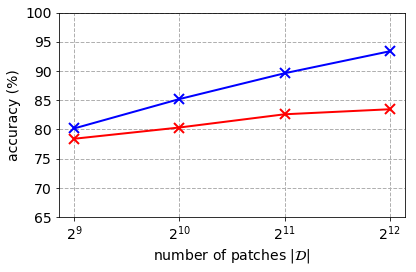
\includegraphics[width=0.49\linewidth]{figures/ablation_npatches_large.png}
  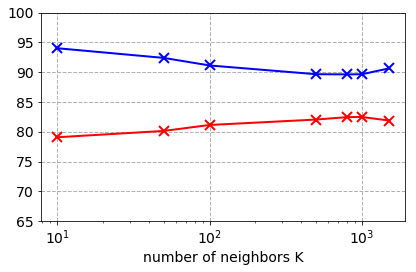
\includegraphics[width=0.49\linewidth]{figures/ablation_K_large.png}
  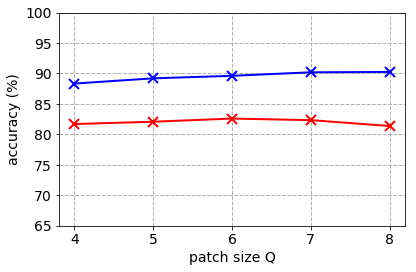
\includegraphics[width=0.49\linewidth]{figures/ablation_Q_large.png}
  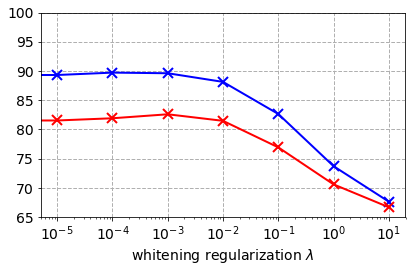
\includegraphics[width=0.49\linewidth]{figures/ablation_lambda_large.png}\\
    \caption{CIFAR-10 ablation experiments, train accuracies in blue, test accuracies in red.
    Number of patches $|\mathcal{D}|$ varies in $\lbrace 512, 1024, 2048, 4096  \rbrace$, number of neighbors $K$ varies in $\lbrace 10, 50, 100, 500, 800, 1000, 1500\rbrace$, patch size $Q$ varies in $\lbrace 4,5,6,7,8 \rbrace$, whitening regularization $\lambda$ varies in $\lbrace0, 10^{-5}, 10^{-4}, 10^{-3}, 10^{-2}, 10^{-1}, 1, 10 \rbrace$. }
    \label{fig:ablation_study_highres}
\end{figure}


\section{Intrinsic dimension estimate}

The following estimate of the intrinsic dimension $d_{\rm int}$ is introduced in \cite{Levina:2004} as follows
\begin{align}
	d_{\rm int}(p) = \left( \frac{1}{K-1} \sum_{k=1}^{K-1}\log \frac{\tau_K(p)}{\tau_k(p)} \right)^{-1} \, ,
\end{align}
where $\tau_k(p)$ is the euclidean distance between the patch $p$ and it's $k$-th nearest neighbor int  the training set.

\end{document}
